\chapter{Results and Discussion}
\label{sec:results}

\section{Effect of Pre-processing Images}
\todo[inline]{Compare tomo\_00058 denoising with and without cropping. Without cropping similar results to early stages of denoising cropped (i.e. poor and not converged). }

\cref{fig:uncroppeddenoising,fig:croppeddenoising}.

\begin{figure}[htbp]
  \centering
  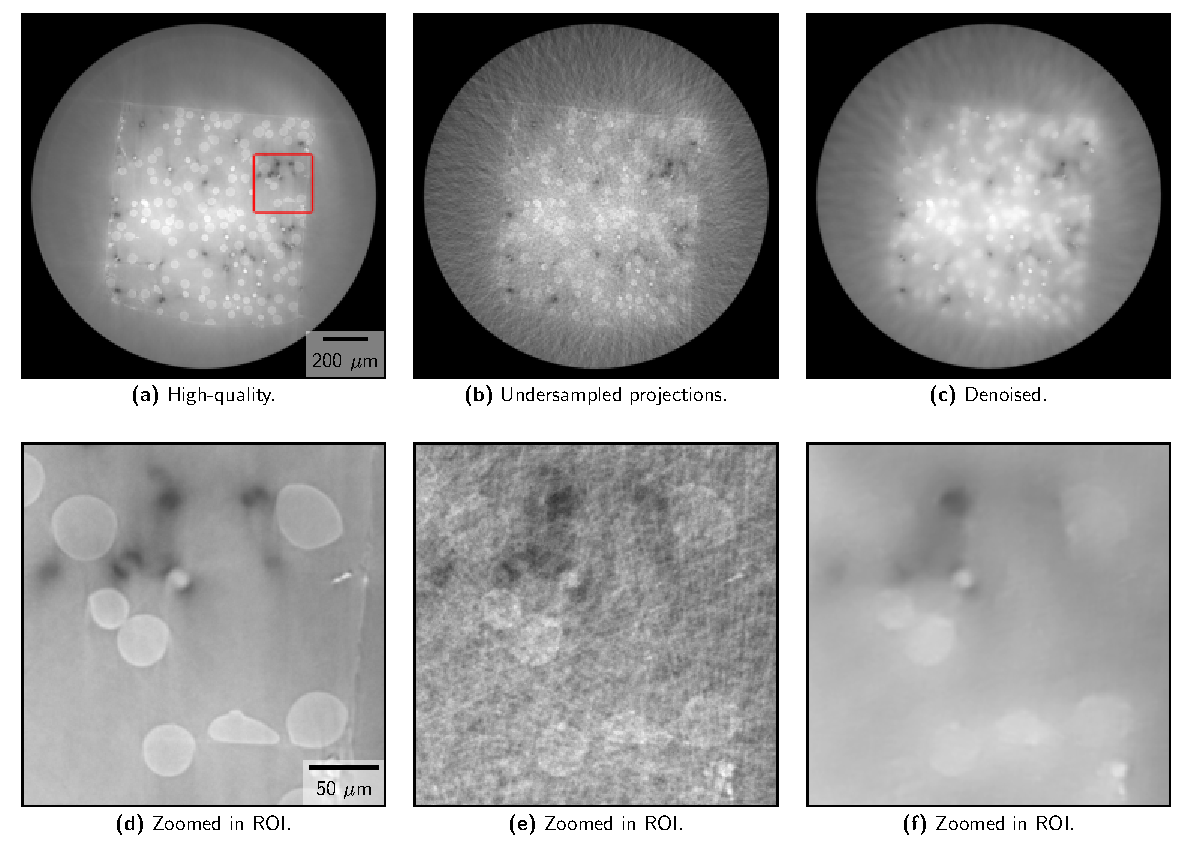
\includegraphics[width=.9\textwidth]{figures/uncroppeddenoising.pdf}
  \caption[Non-cropped image denoising]{Denoising of non-cropped dataset tomo\_00058. Images d), e), and f) are zoomed in \acrshort{roi}s of images a), b), and c) respectively. The \acrshort{roi} is marked in a). }
  \label{fig:uncroppeddenoising}
\end{figure}

\begin{figure}[htbp]
  \centering
  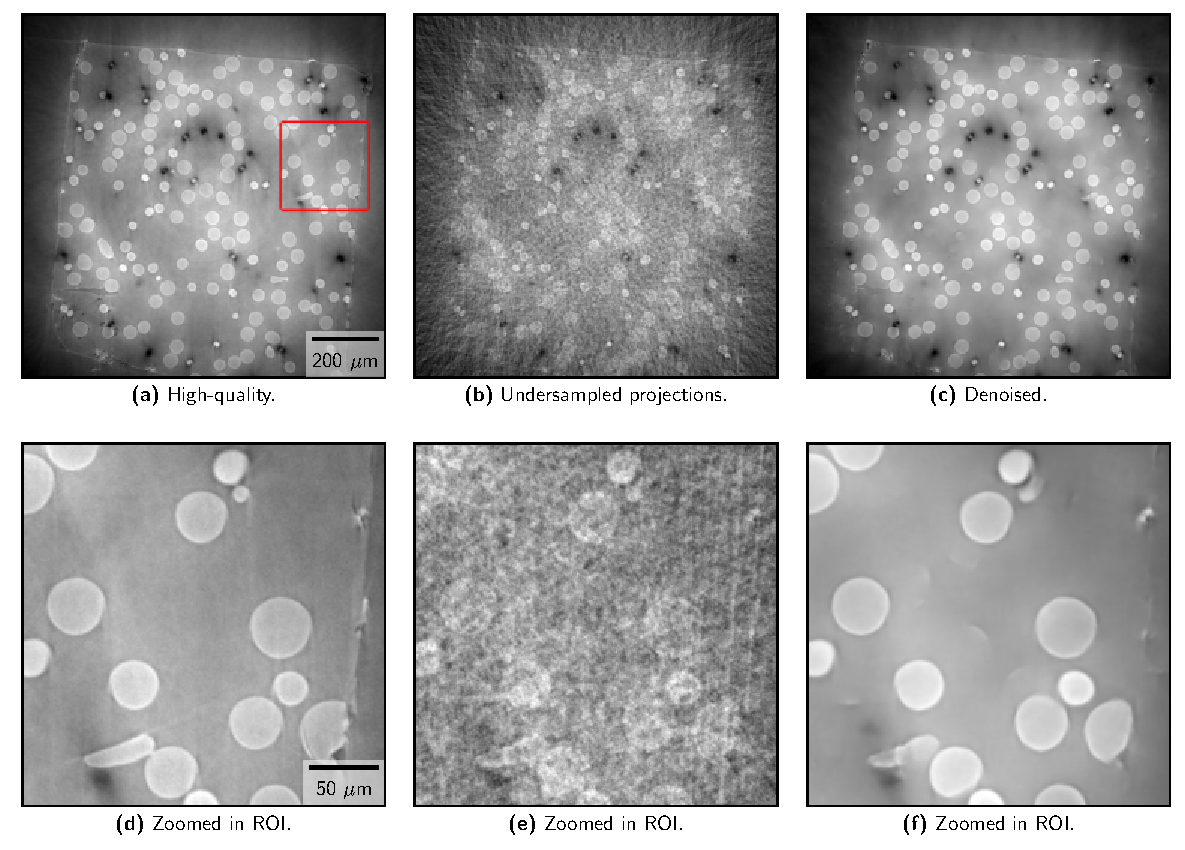
\includegraphics[width=.9\textwidth]{figures/croppeddenoising.pdf}
  \caption[Cropped image denoising]{Denoising of cropped dataset tomo\_00058. Images d), e), and f) are zoomed in \acrshort{roi}s of images a), b), and c) respectively. The \acrshort{roi} is marked in a). }
  \label{fig:croppeddenoising}
\end{figure}


\section{Hyperparameter and Loss Function Changes}
\todo[inline]{Show difference in tomo\_00058 denoising for different loss functions / weights (and hyperparameters?)}

\todo[inline]{Line plot of gt, ns, MSE denoising, log-cosh denoising. Multiple lines around the images?}

\todo[inline]{SSIM and MSE evolution of arbitrary slice. }

\section{Different Amounts of Noise}
\todo[inline]{Different levels of noise / projection subsamplings (8,16,32,48). }
\todo[inline]{Plot of the images with zoomed in ROIs. }
\todo[inline]{Plot showing improvement in SSIM for different levels of noise. }
\todo[inline]{Line plot for different levels of noise? }

\cref{tab:missingwedgessim}, and \cref{fig:tomo00058missingwedgecomparison,fig:tomo00058missingwedgecomparisondenoised,fig:differentnoiselineplot1,fig:differentnoiselineplot2}. 

\begin{figure}
  \begin{subfigure}[t]{\textwidth}
    \centering
    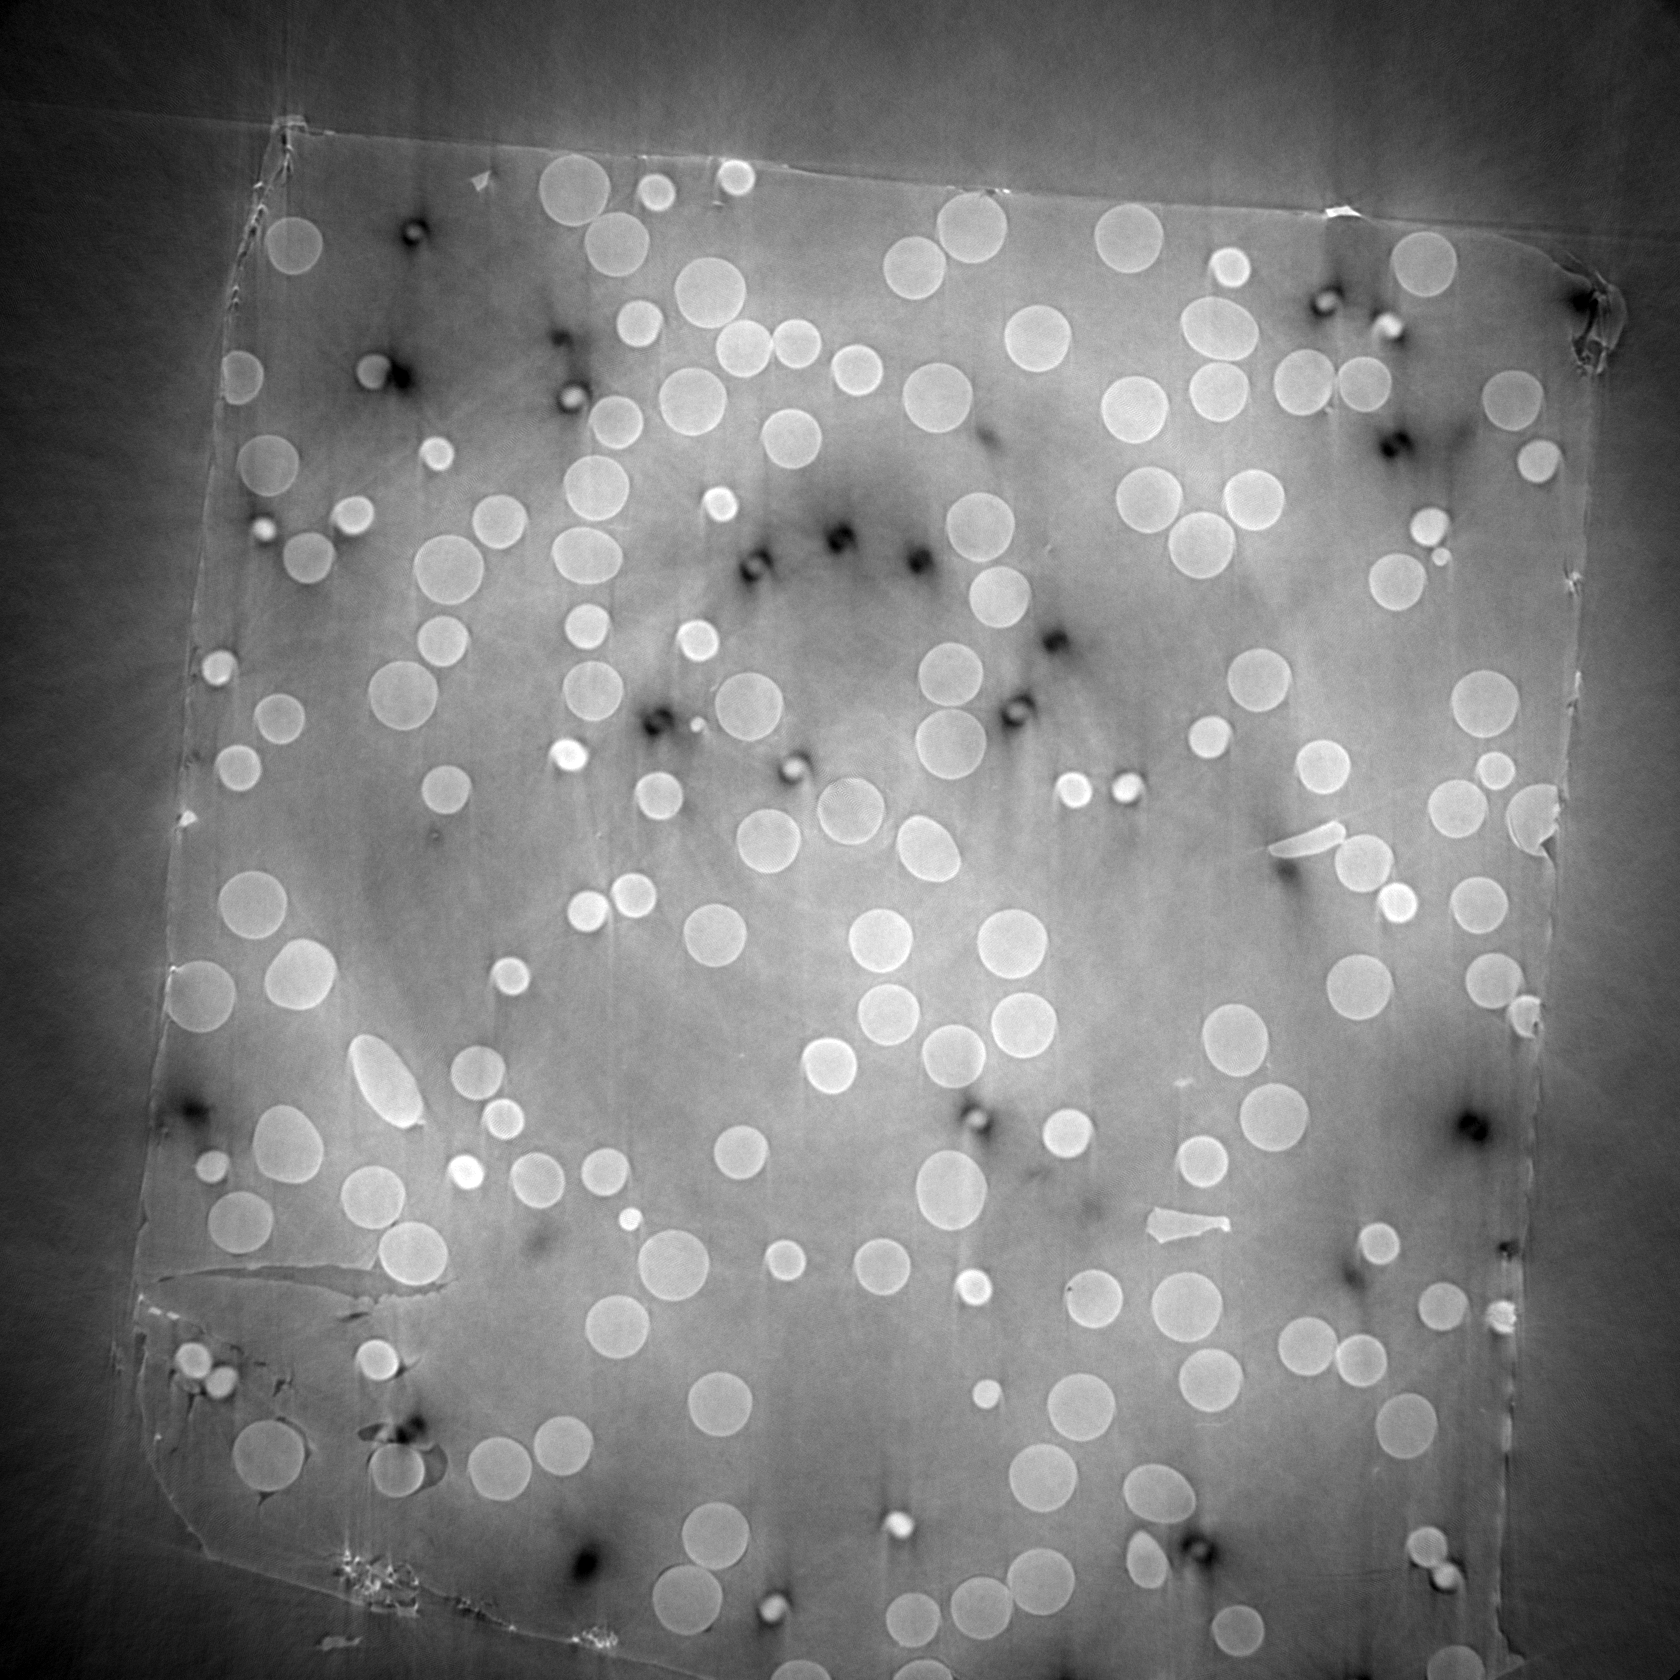
\includegraphics[width=.45\textwidth]{figures/gt32.png}
    \caption{High-quality. }
  \end{subfigure}

  \medskip

  \begin{subfigure}[t]{.45\textwidth}
    \centering
    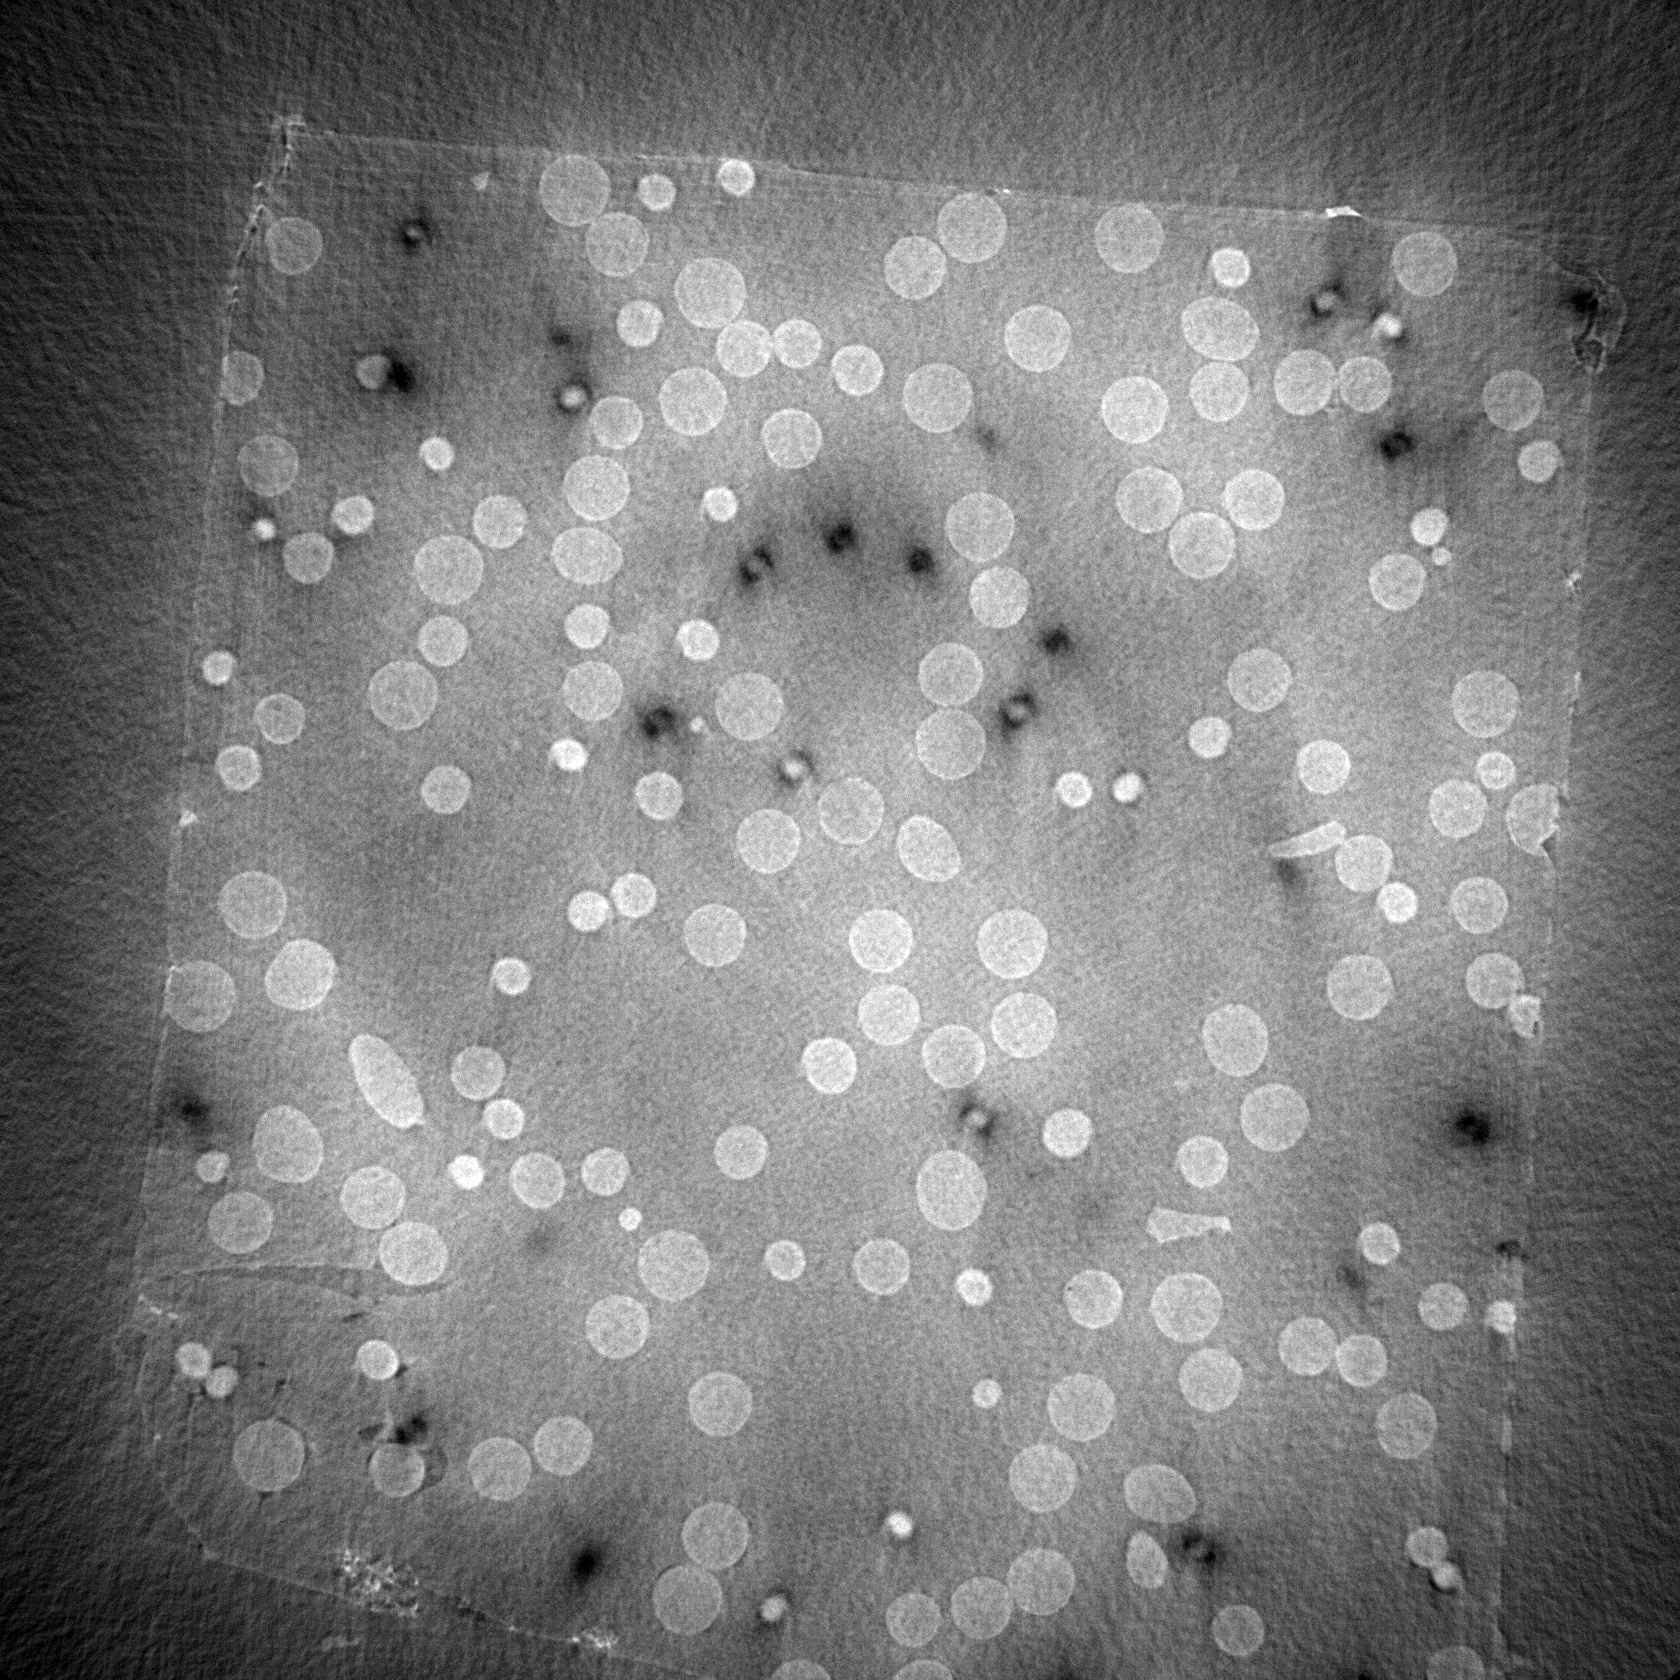
\includegraphics[width=\linewidth]{figures/ns8.png}
    \caption{Subsampling factor 8. }
  \end{subfigure}
  \hfill
  \begin{subfigure}[t]{.45\textwidth}
    \centering
    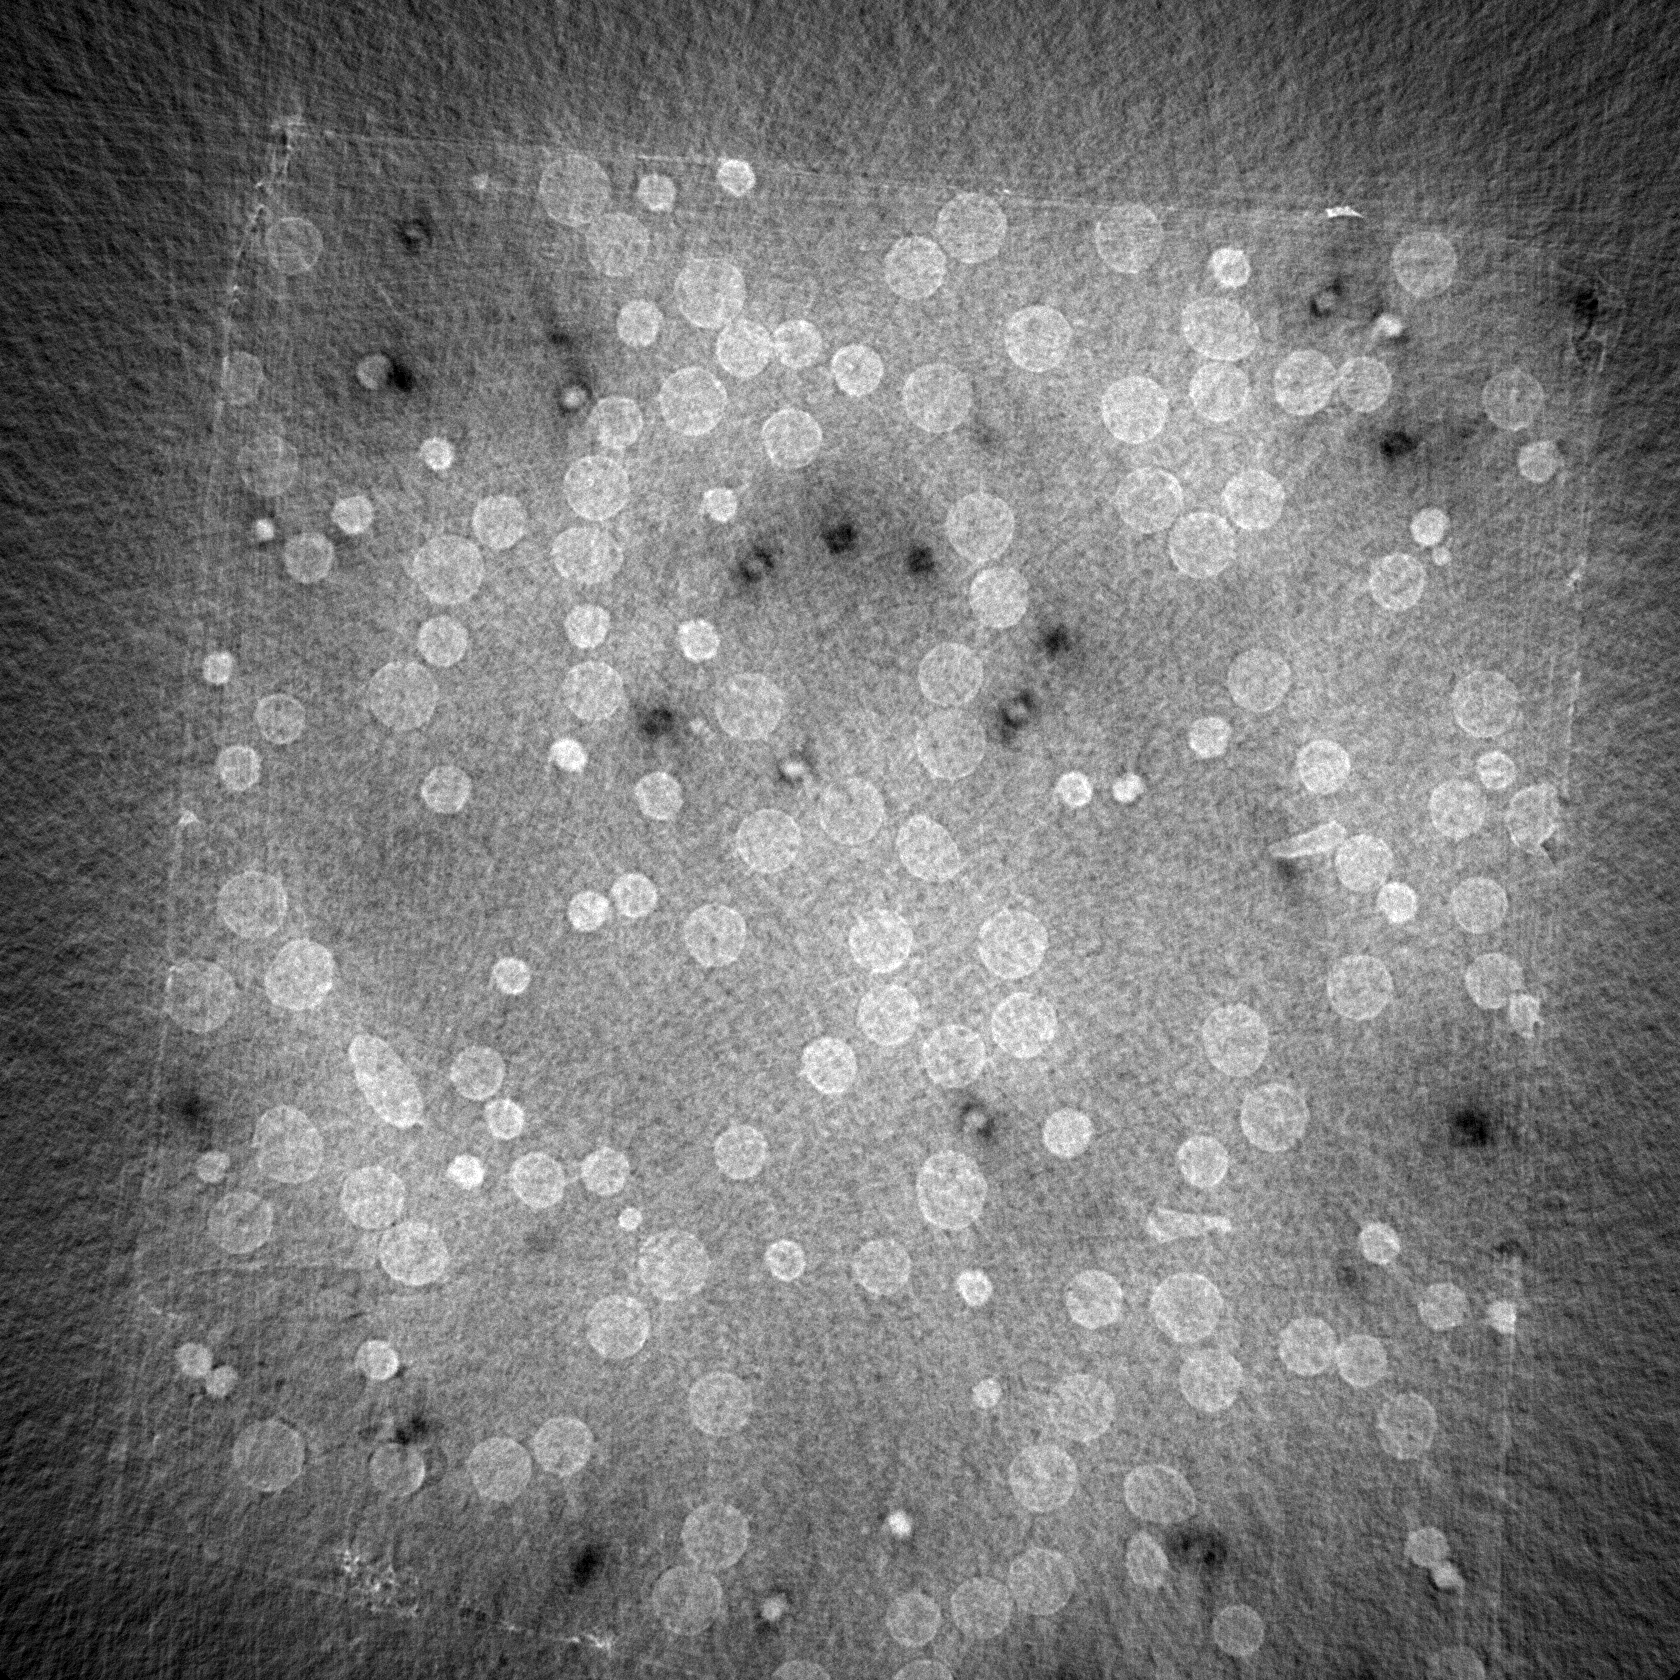
\includegraphics[width=\linewidth]{figures/ns16.png}
    \caption{Subsampling factor 16. }
  \end{subfigure}

  \medskip

  \begin{subfigure}[t]{.45\textwidth}
    \centering
    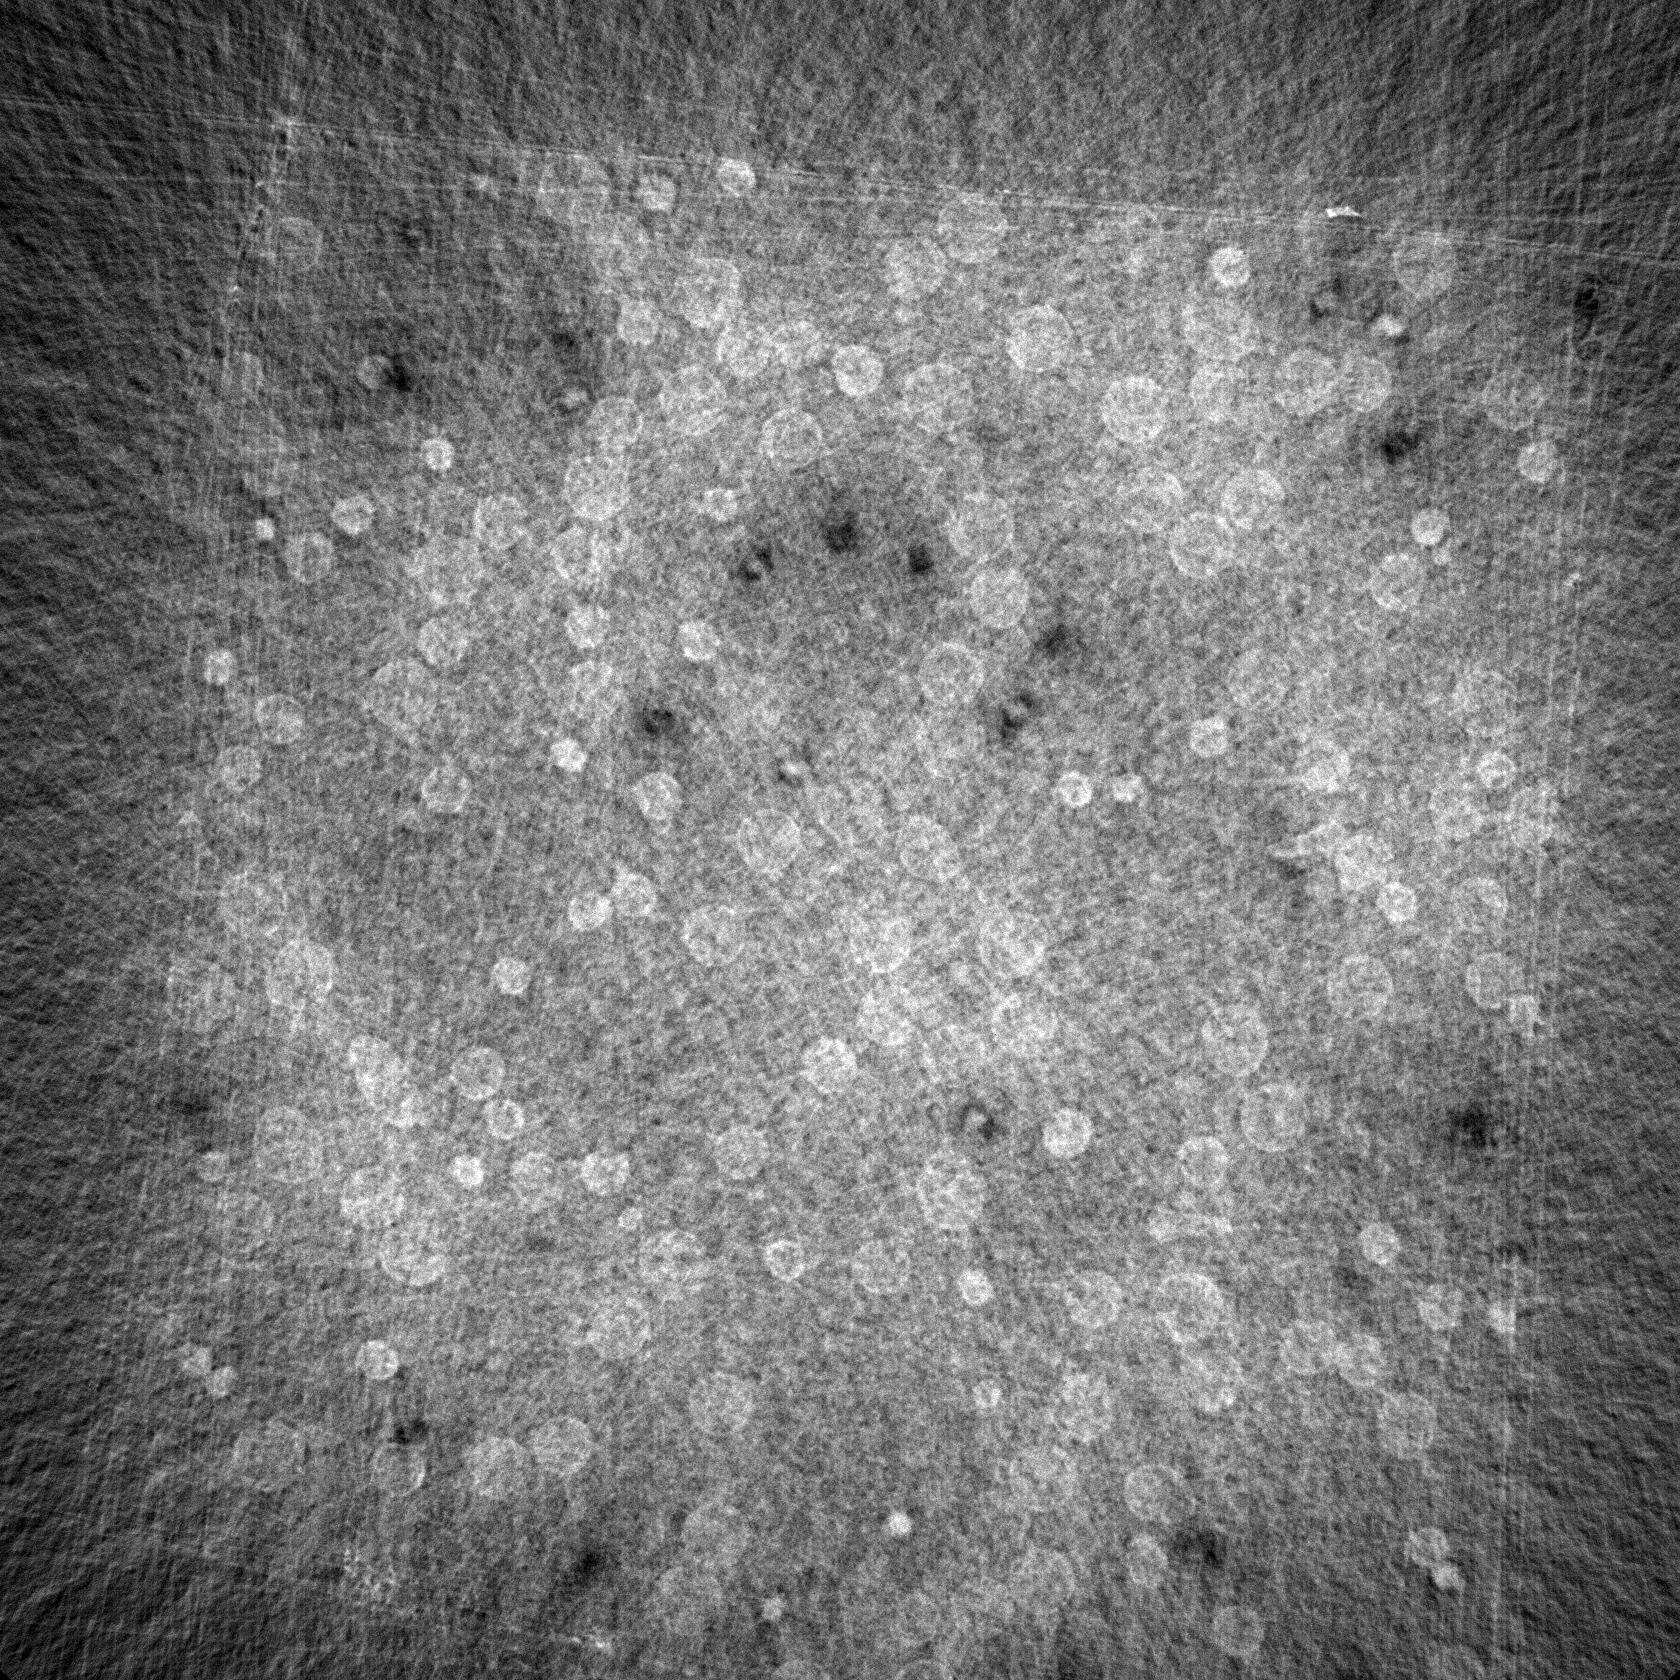
\includegraphics[width=\linewidth]{figures/ns32.png}
    \caption{Subsampling factor 32. }
  \end{subfigure}
  \hfill
  \begin{subfigure}[t]{.45\textwidth}
    \centering
    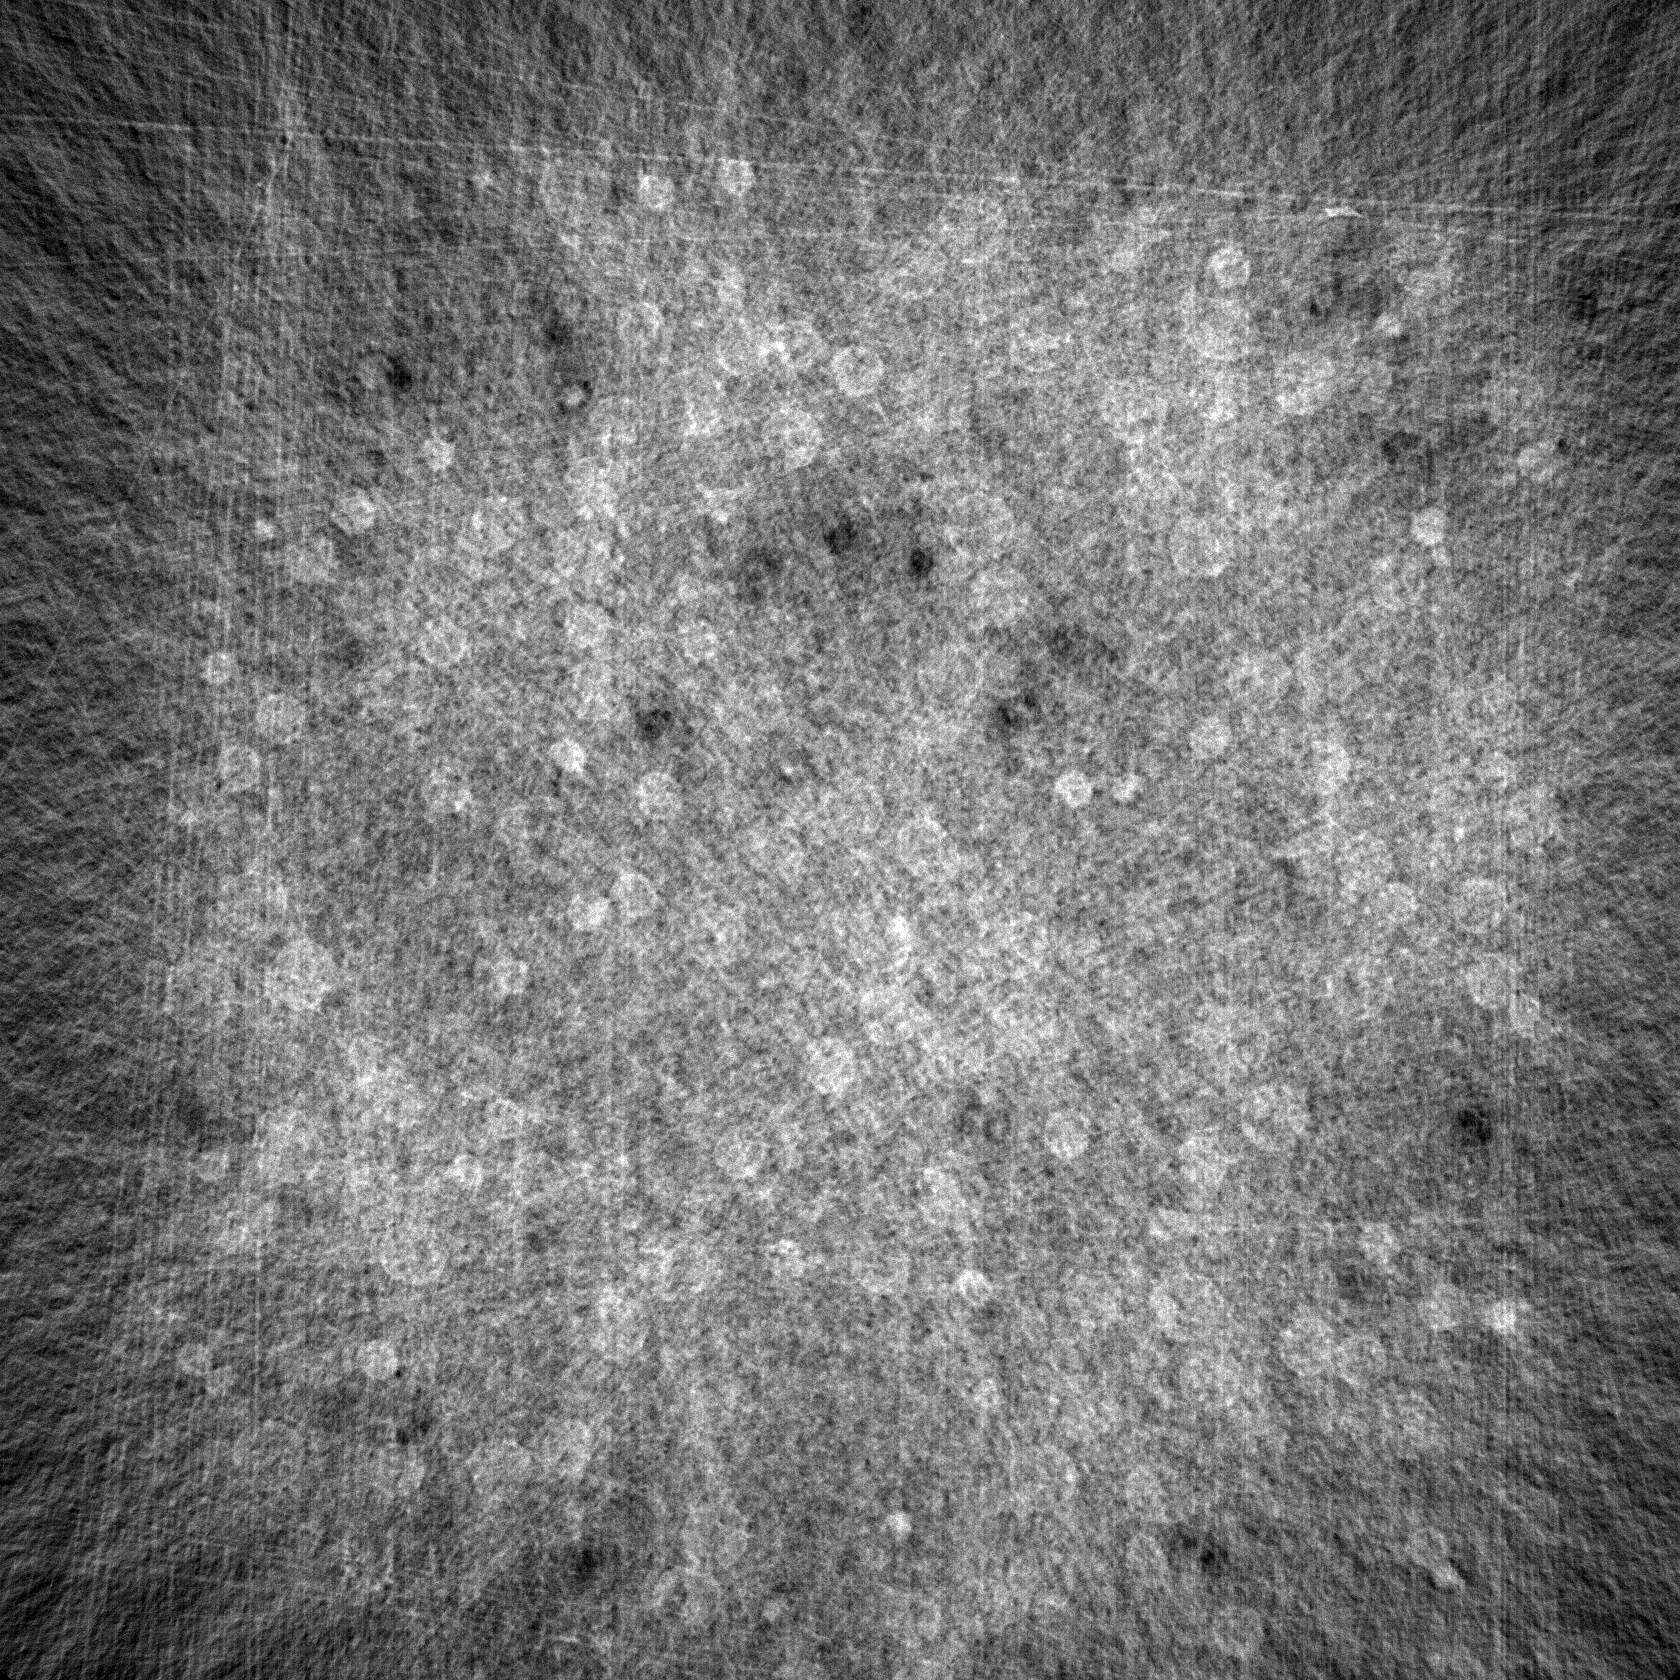
\includegraphics[width=\linewidth]{figures/ns48.png}
    \caption{Subsampling factor 48. }
  \end{subfigure}
  \caption[Four different levels of missing wedge noise]{Comparison of different levels of missing wedge noise on the tomo\_00058 dataset. The four noisy images have been reconstructed with \acrshort{fbp} with different levels of subsampling of the projections, leading to noise. The number of projections corresponding to a given subsampling factor can be seen in \cref{tab:projectionsubsampling}. }
  \label{fig:tomo00058missingwedgecomparison}
\end{figure}


\begin{figure}
  \begin{subfigure}[t]{.45\textwidth}
    \centering
    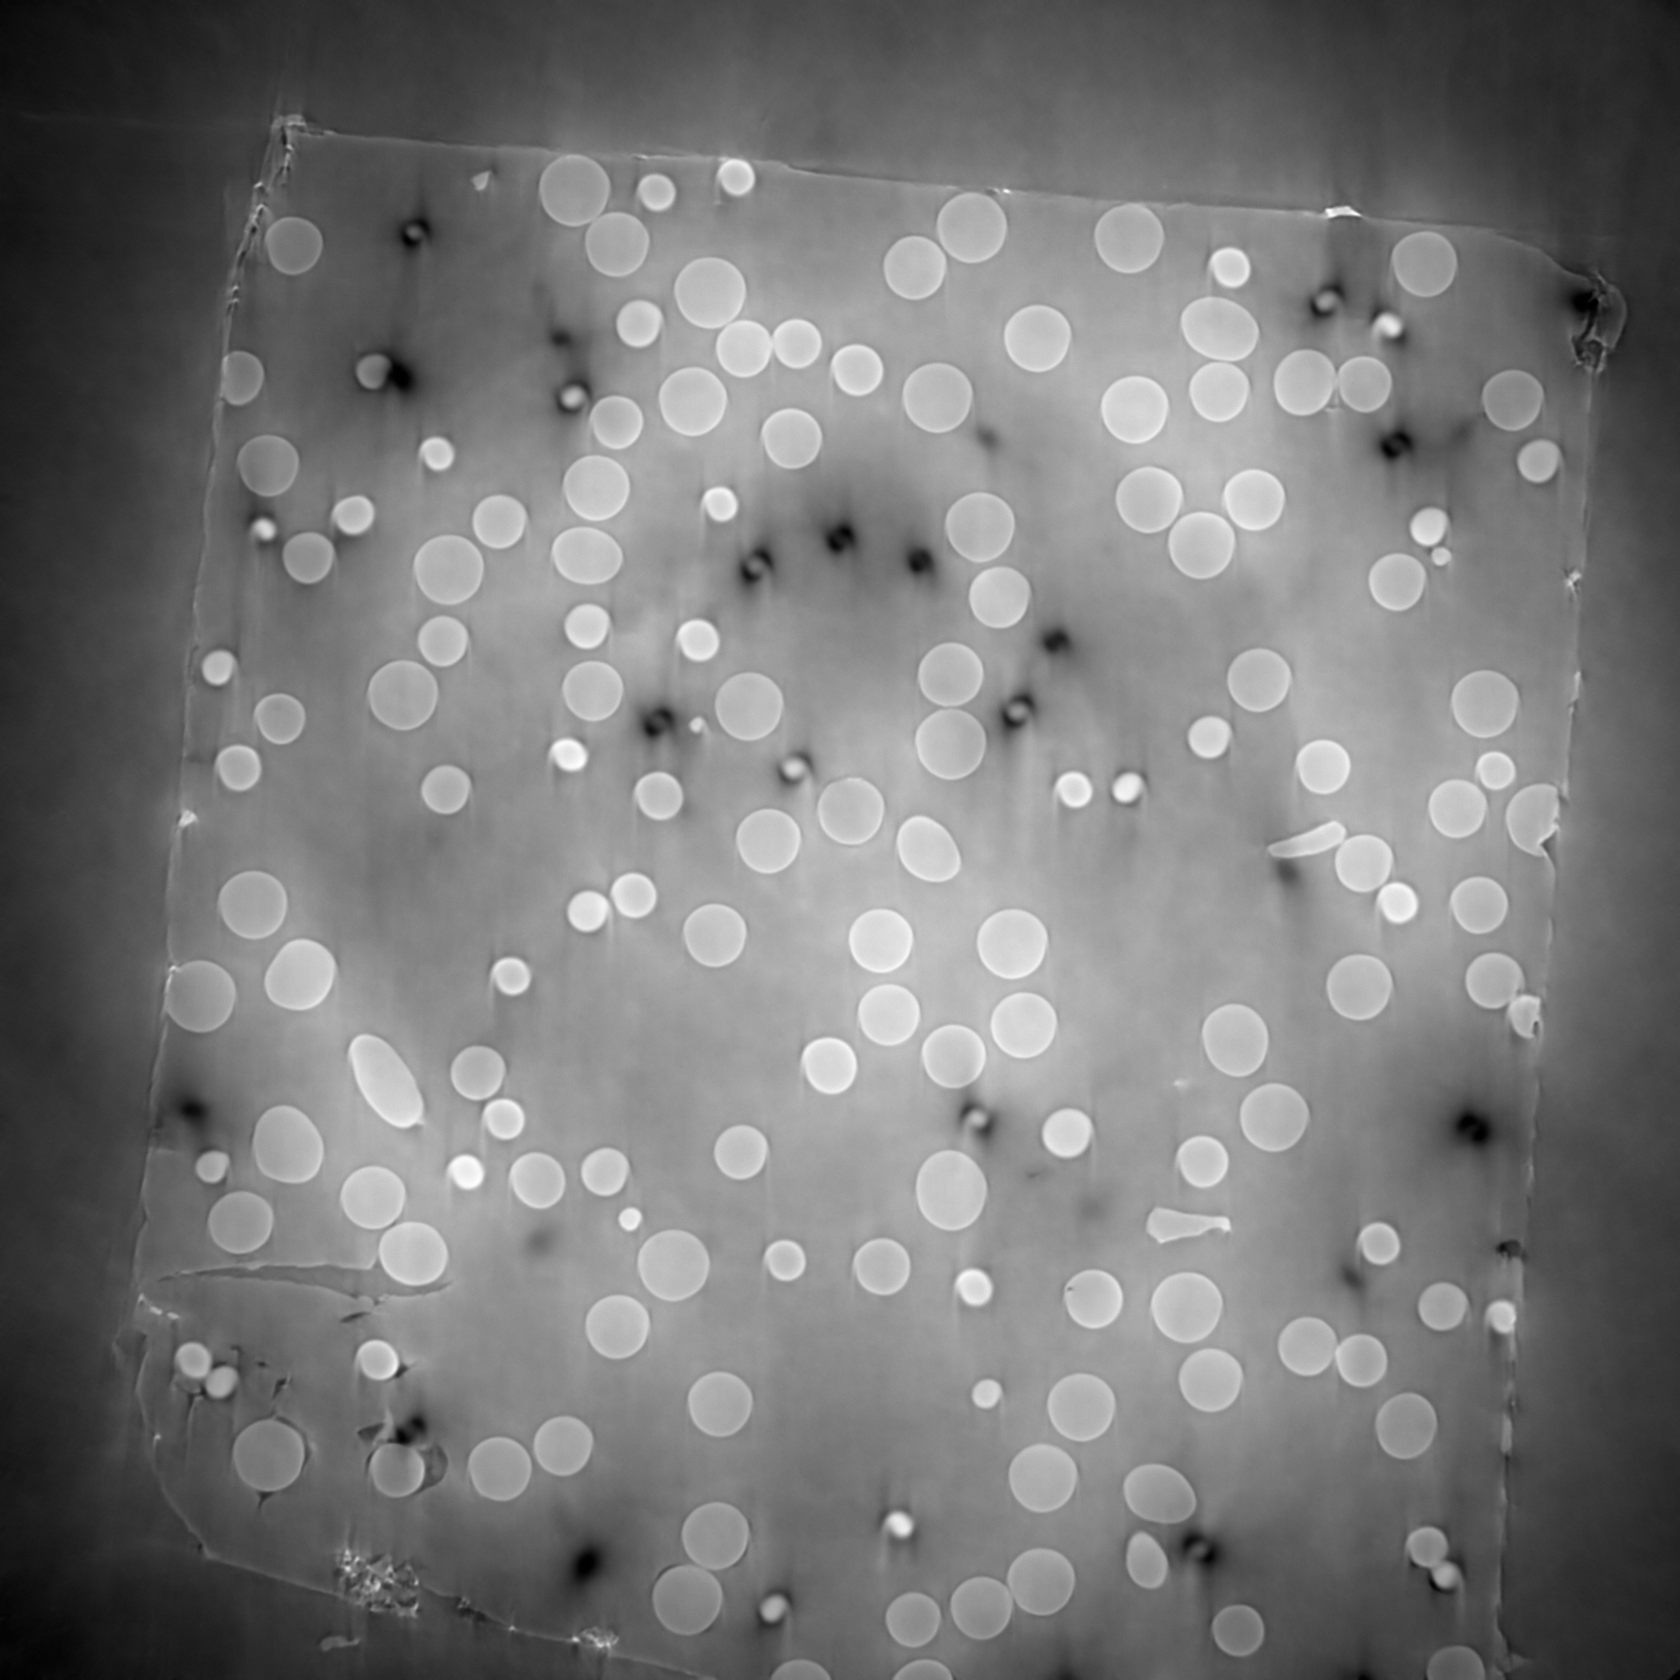
\includegraphics[width=\linewidth]{figures/ns8it100000itd4mse035logcosh3.png}
    \caption{Subsampling factor 8. }
  \end{subfigure}
  \hfill
  \begin{subfigure}[t]{.45\textwidth}
    \centering
    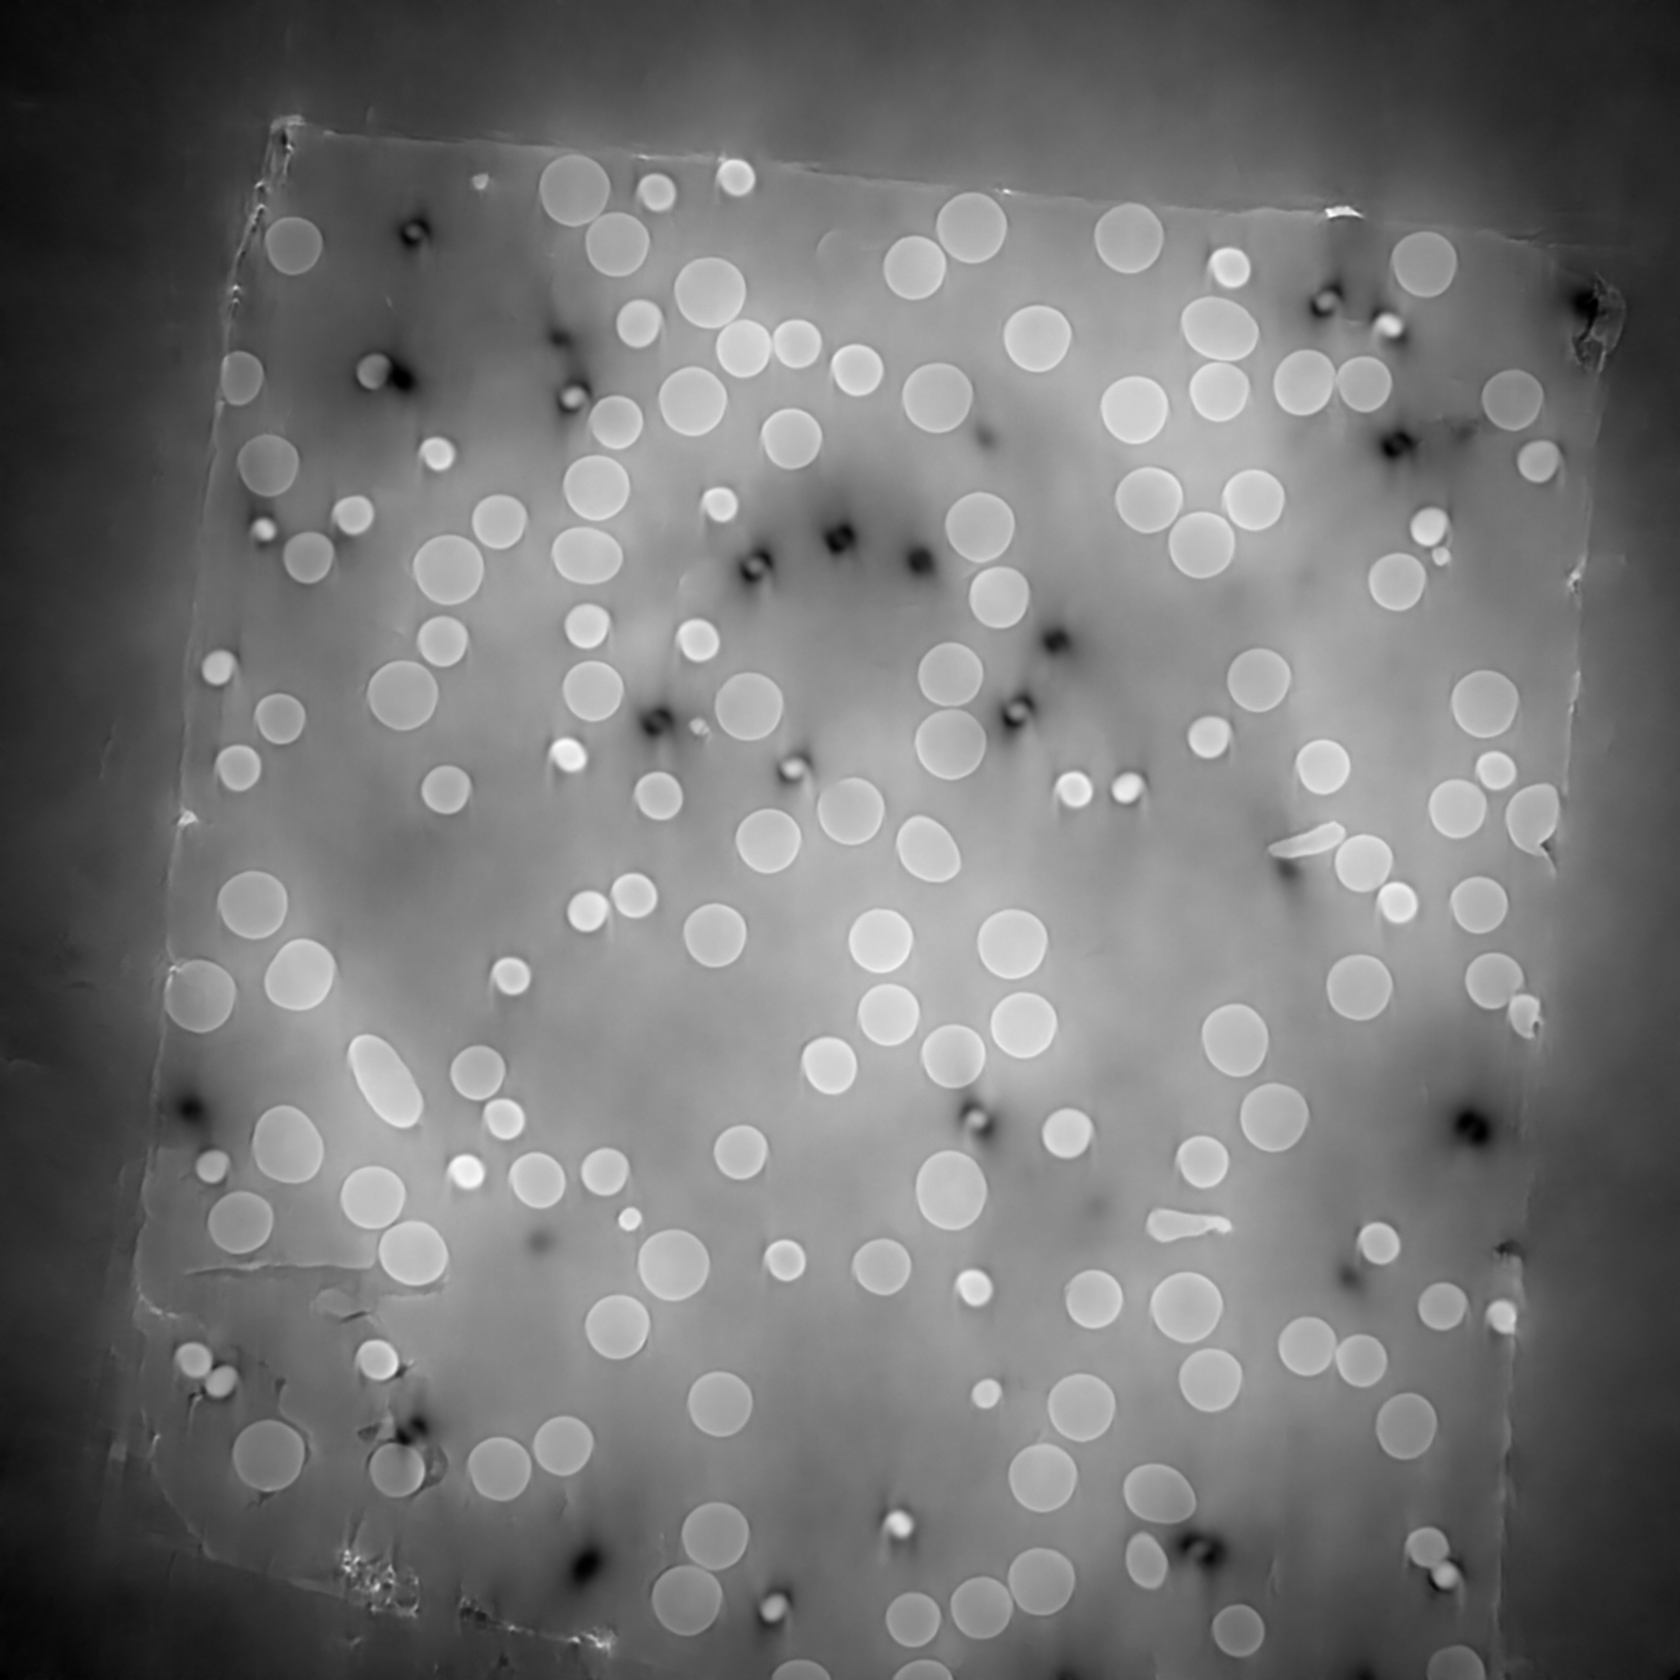
\includegraphics[width=\linewidth]{figures/ns16it100000itd4mse035logcosh3.png}
    \caption{Subsampling factor 16. }
  \end{subfigure}

  \medskip

  \begin{subfigure}[t]{.45\textwidth}
    \centering
    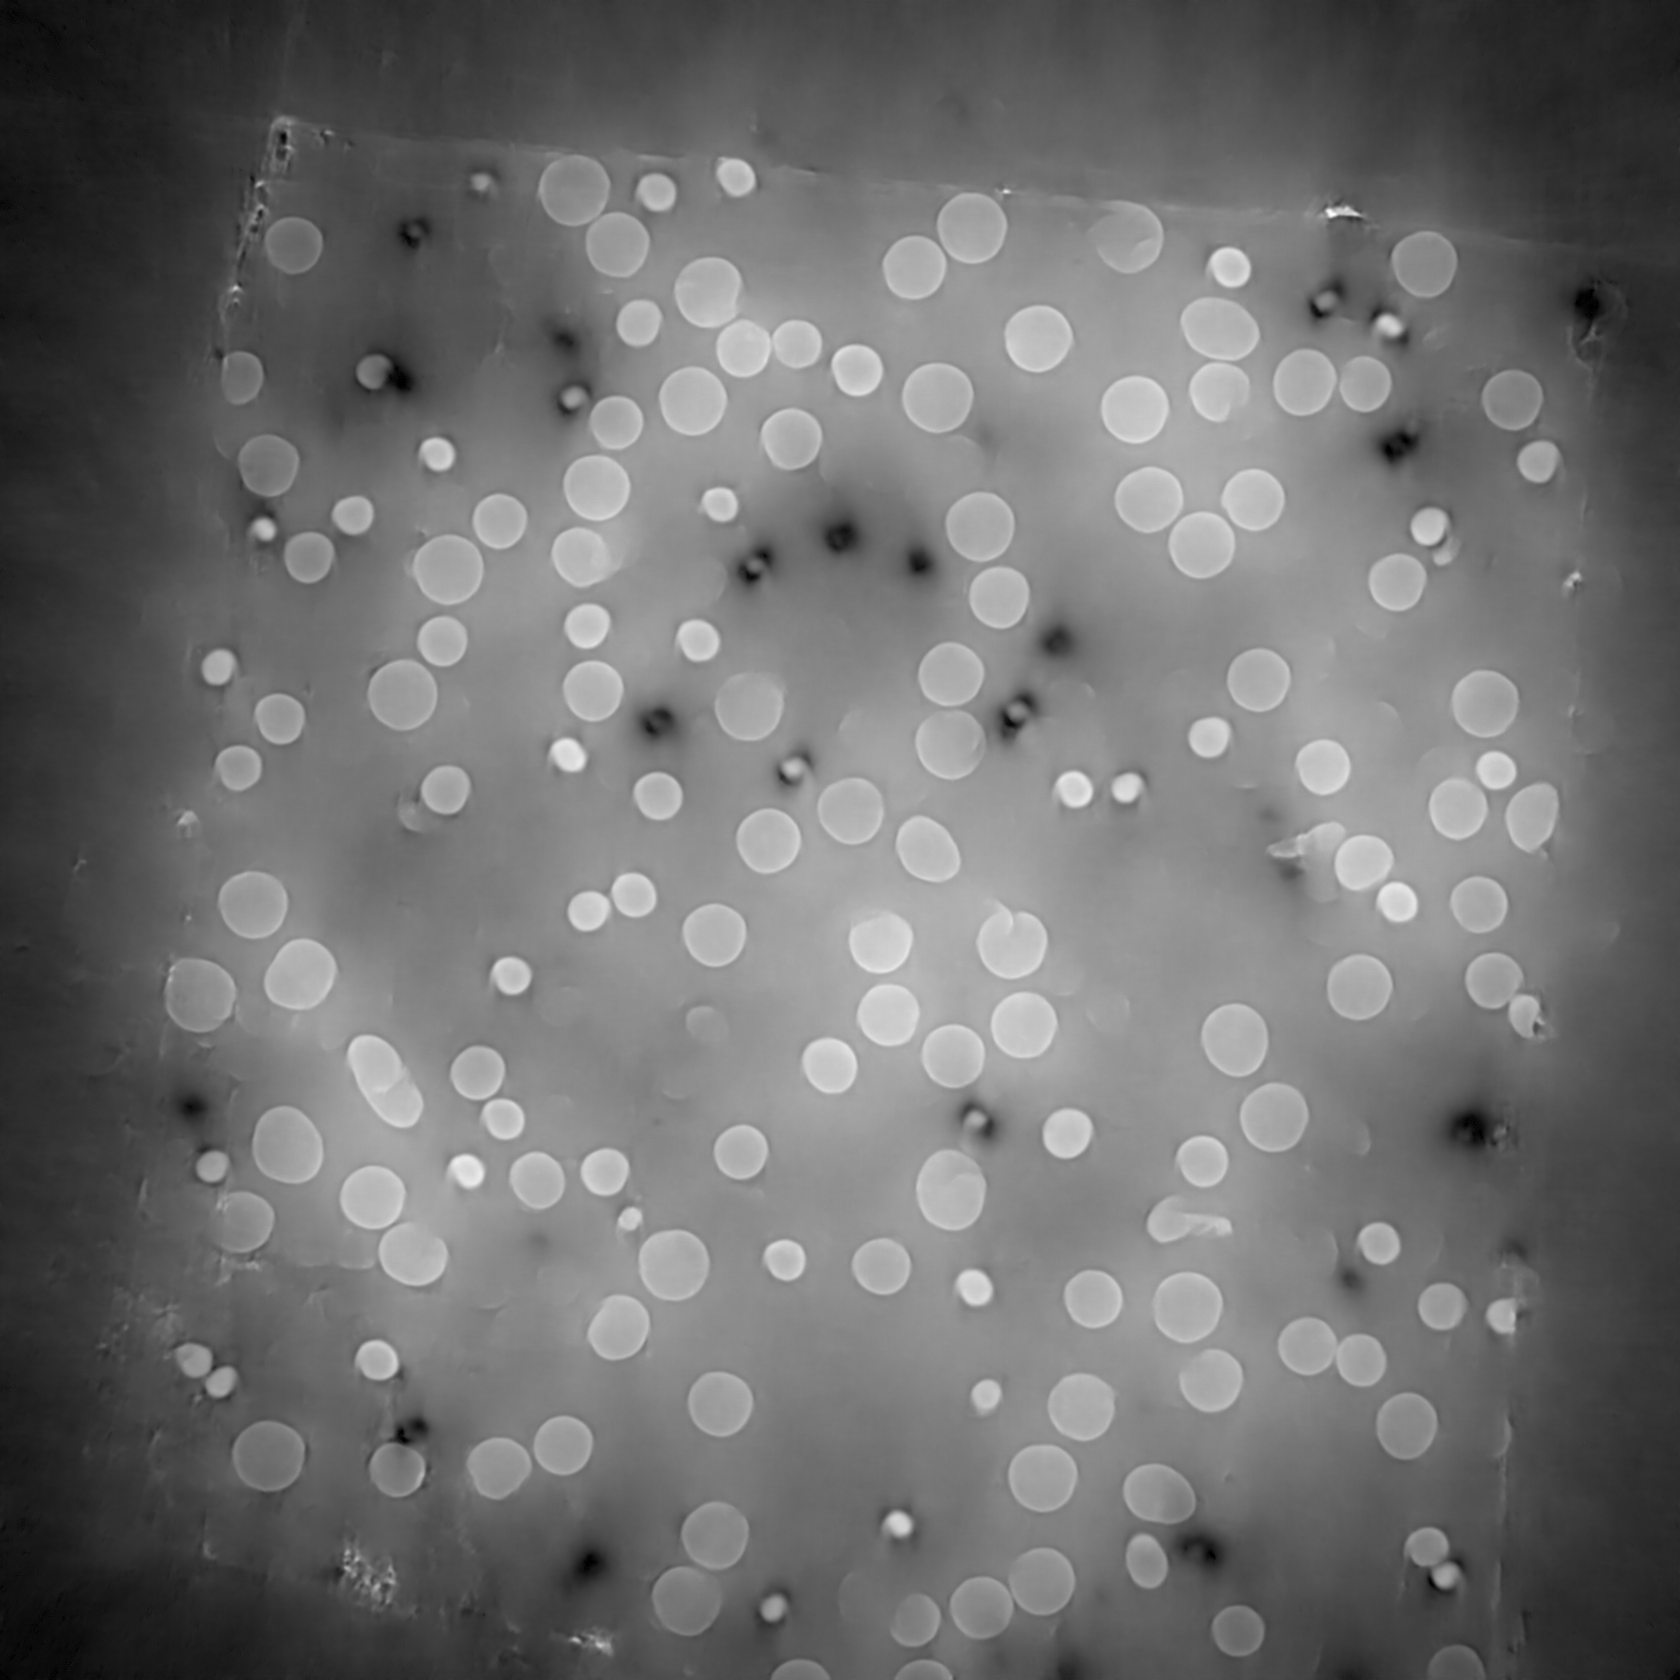
\includegraphics[width=\linewidth]{figures/ns32it100000itd4mse035logcosh3.png}
    \caption{Subsampling factor 32. }
  \end{subfigure}
  \hfill
  \begin{subfigure}[t]{.45\textwidth}
    \centering
    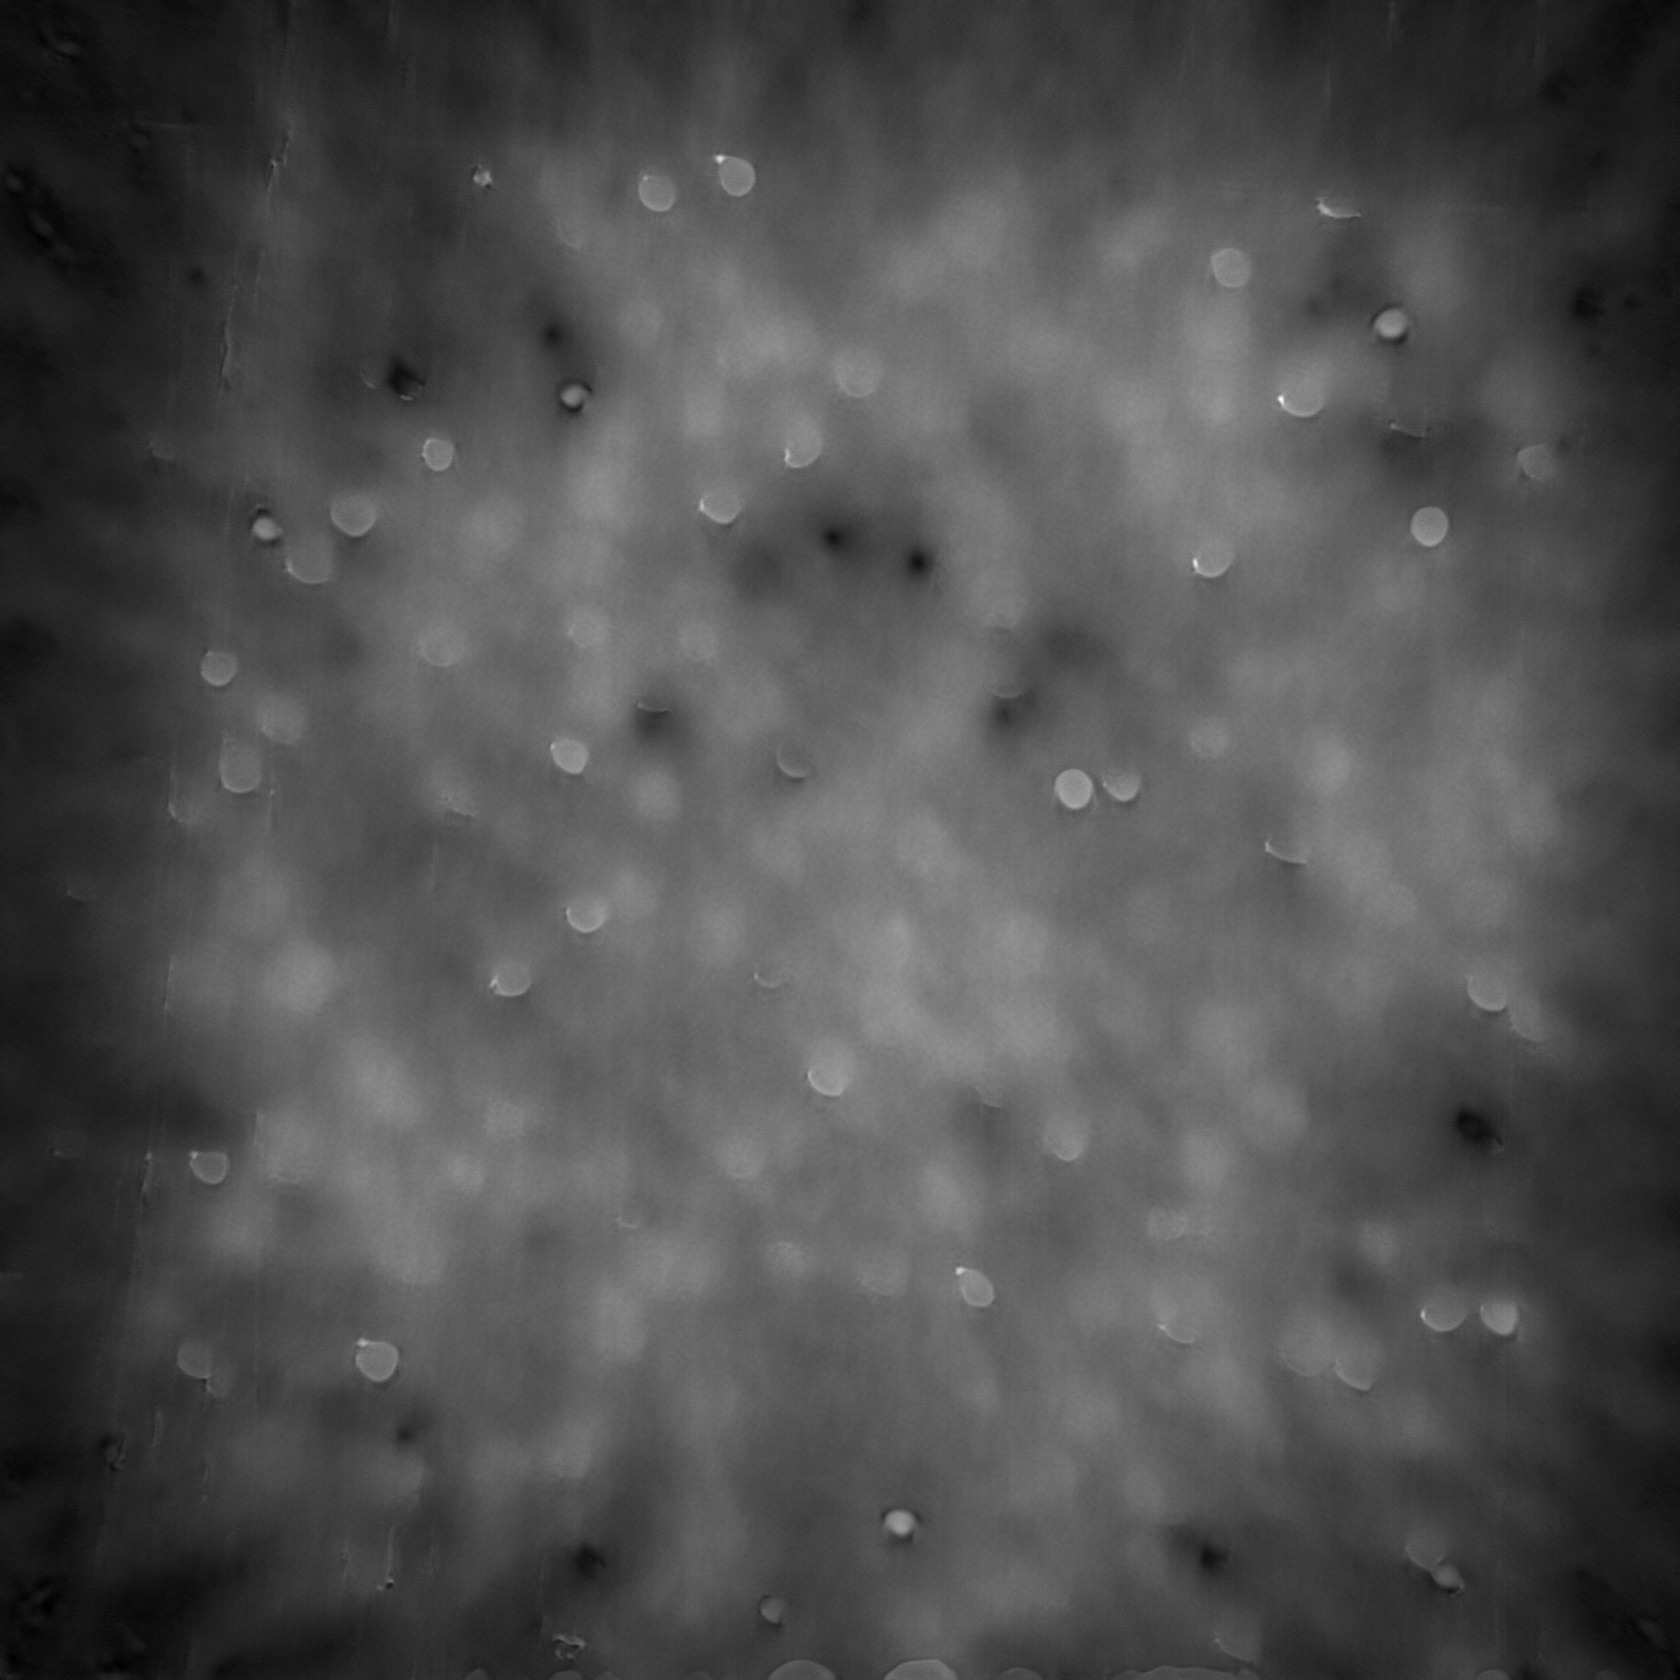
\includegraphics[width=\linewidth]{figures/ns48it100000itd4mse035logcosh3.png}
    \caption{Subsampling factor 48. }
  \end{subfigure}
  \caption[Denoising of four different levels of missing wedge noise]{Comparison of denoising of different levels of missing wedge noise on the tomo\_00058 dataset, where the corresponding noisy images can be seen in \cref{fig:tomo00058missingwedgecomparison}. The denoising was done with TomoGAN using a loss function containing \acrshort{mse}, log-cosh, VGG, and adversarial loss components, a depth of 1, and the network was trained for $100 000$ iterations. }
  \label{fig:tomo00058missingwedgecomparisondenoised}
\end{figure}


\begin{table}[htbp]
  \centering
  \caption[SSIM for different levels of simulated missing wedge noise and corresponding values after denoising]{Overview of \acrshort{ssim} for different levels of simulated missing wedge noise on the tomo\_00058 dataset. The missing wedge noise was simulated by subsampling the number of projections by a factor as given in the subsampling factor column, which results in a number of projections as given in \cref{tab:projectionsubsampling}. All denoising was done with TomoGAN using a loss function containing \acrshort{mse}, log-cosh, VGG, and adversarial loss components, a depth of 1, and the network was trained for $100 000$ iterations. }
  \label{tab:missingwedgessim}
  \begin{tabular}{lllll}
  \hline
  \multirow{2}{*}{Subsampling factor} & \multicolumn{2}{c}{\acrshort{ssim}} & \multicolumn{2}{c}{\acrshort{mse}}  \\
  {} & Noisy & Denoised & Noisy & Denoised \\
  \hhline{=====}
  %\hline 
  $1$  & $1.0$ & $-$ & $0.0$ & $-$ \\
  $8$  & $0.492$ & $0.842$ & $148.3$ & $33.3$ \\
  $16$ & $0.335$ & $0.816$ & $348.5$ & $74.9$ \\
  $32$ & $0.233$ & $0.789$ & $704.4$ & $210.8$ \\
  $48$ & $0.193$ & $0.657$ & $976.6$ & $2362.6$ \\
  \hline
  \end{tabular}
\end{table}

\begin{figure}[htbp]
  \centering
  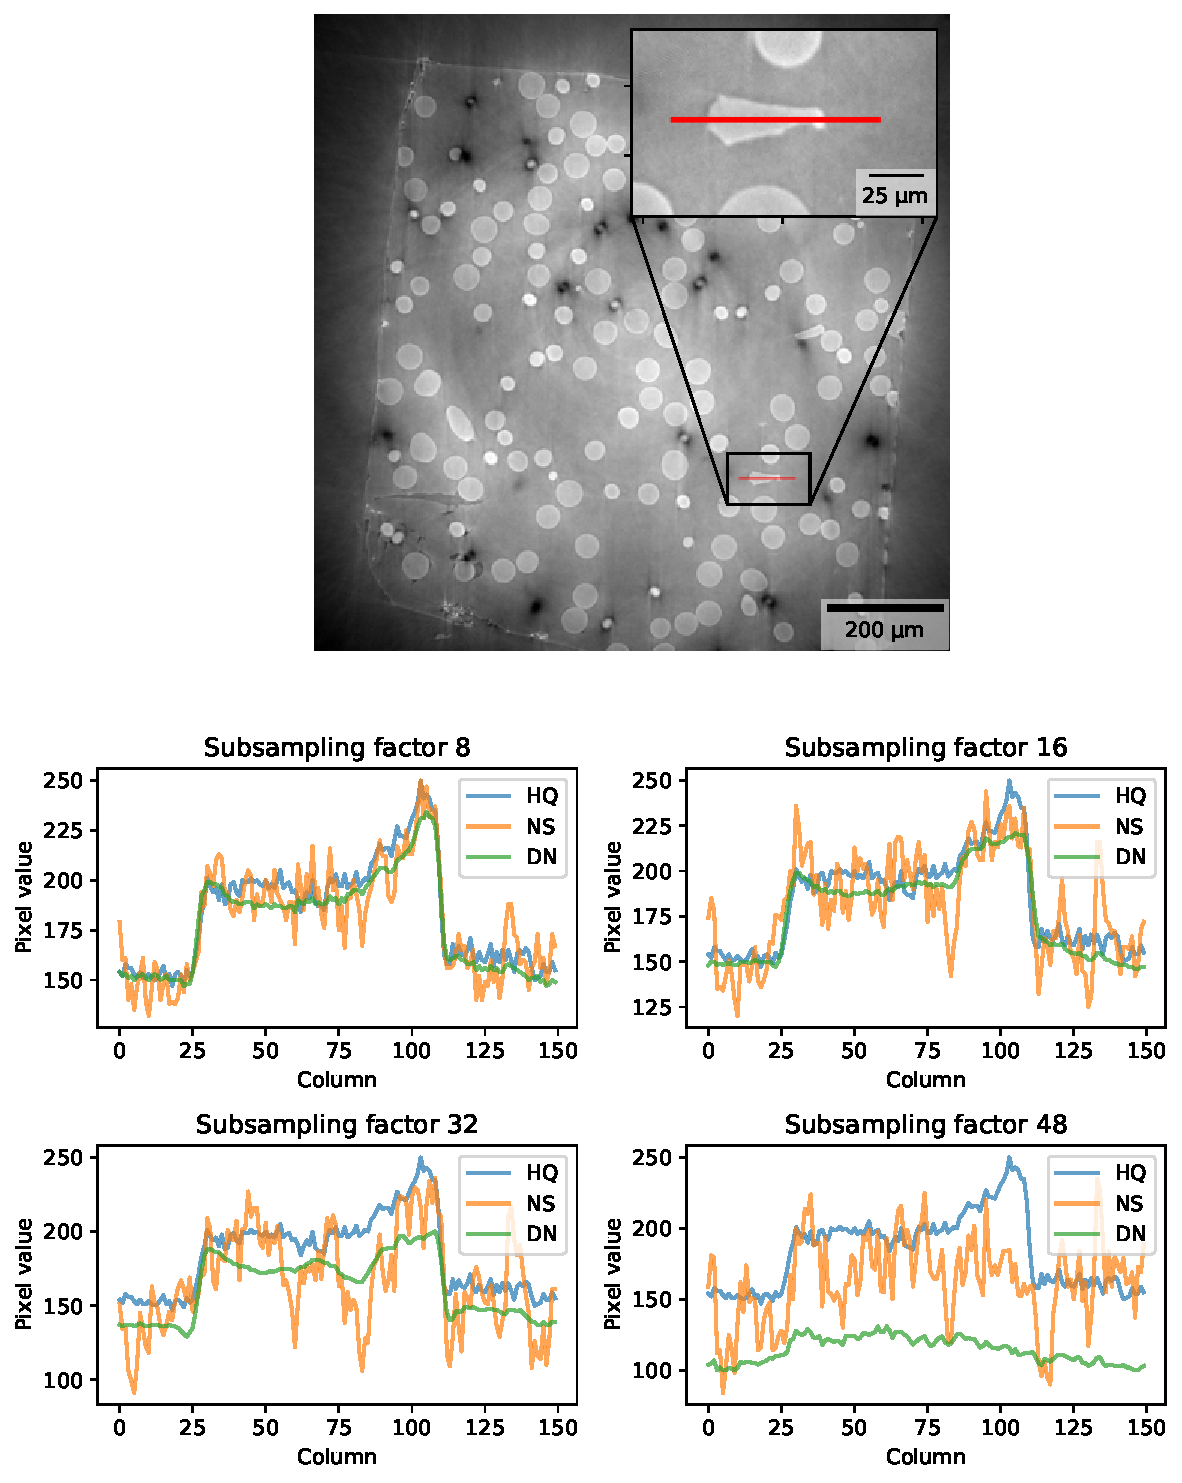
\includegraphics[width=.95\textwidth]{figures/differentnoiselineplot1.pdf}
  \caption[Line plot of denoising of different levels of noise]{The plots show pixel values for 150 pixels on a horizontal line, as shown by the red line on the high-quality image above, for denoising of four different levels of missing wedge noise. HQ corresponds to the high-quality image, NS to the missing wedge noise image, and DN to the denoised image. All denoising was done with TomoGAN using a loss function containing \acrshort{mse}, log-cosh, VGG, and adversarial loss components, a depth of 1, and the network was trained for $100 000$ iterations. }
  \label{fig:differentnoiselineplot1}
\end{figure}

\begin{figure}[htbp]
  \centering
  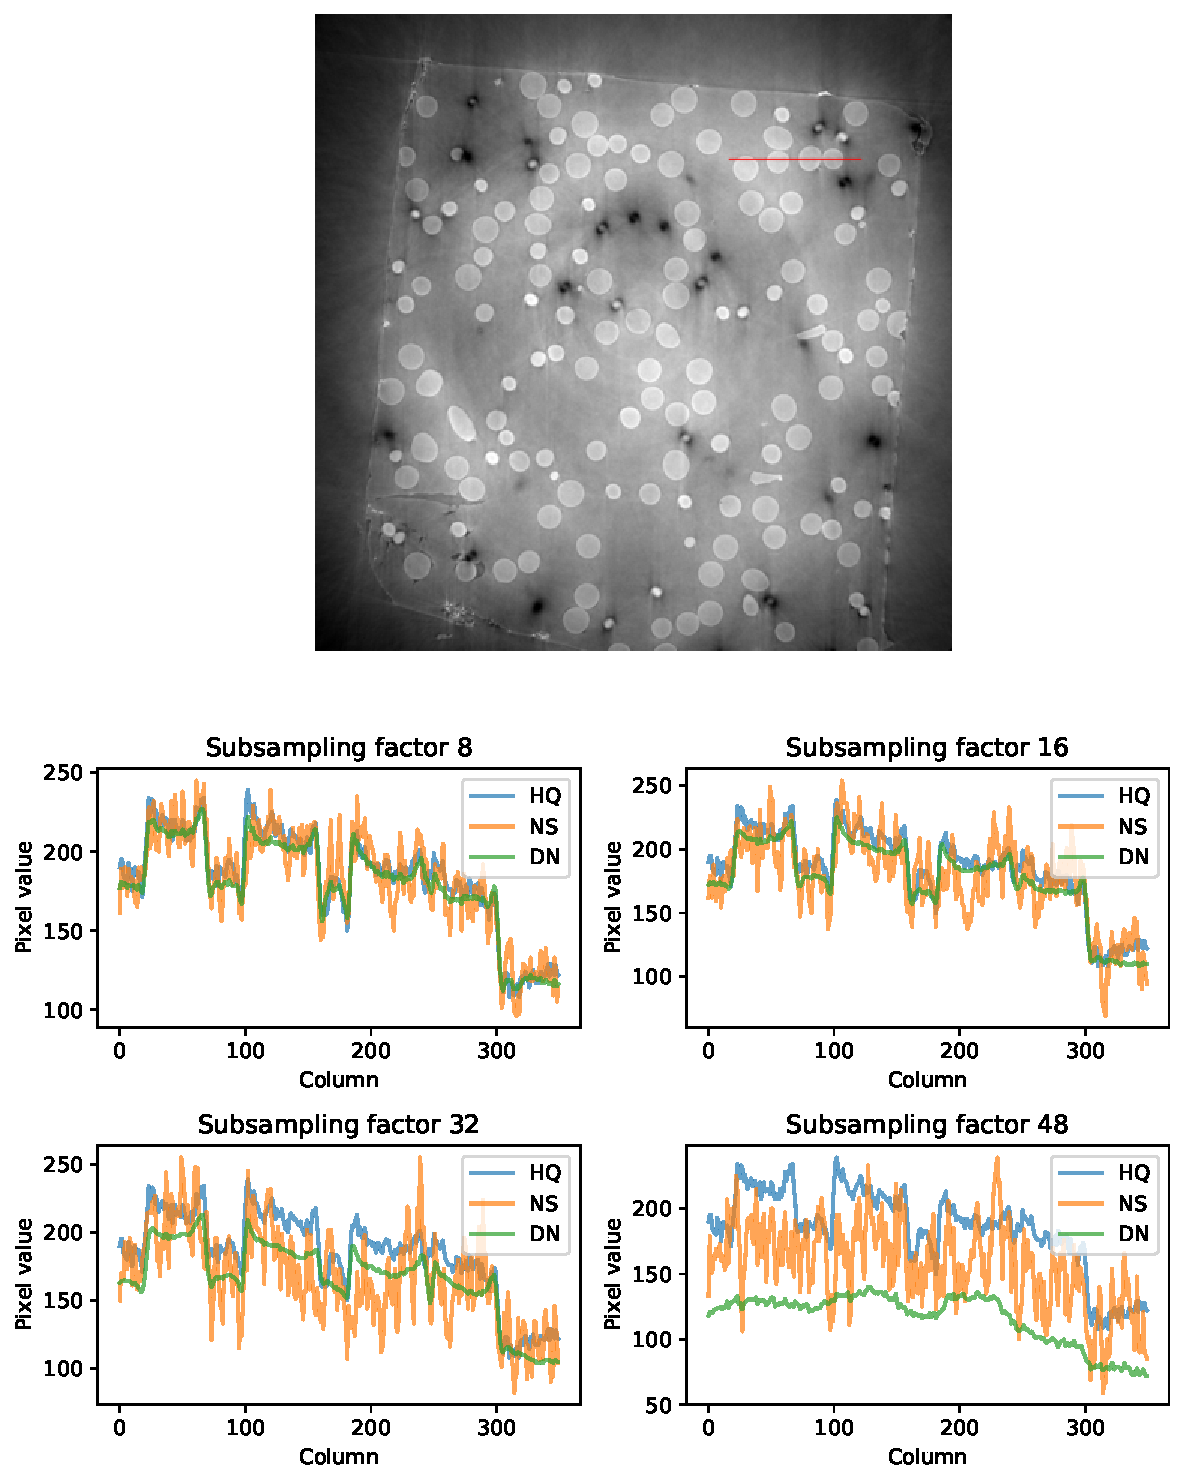
\includegraphics[width=.95\textwidth]{figures/differentnoiselineplot2.pdf}
  \caption[Line plot of denoising of different levels of noise]{The plots show pixel values for 350 pixels on a horizontal line, as shown by the red line on the high-quality image above, for denoising of four different levels of missing wedge noise. Figure elements are as in \cref{fig:differentnoiselineplot1}. }
  \label{fig:differentnoiselineplot2}
\end{figure}

\section{Loss Function Evolution}
\todo[inline]{Plot how loss functions evolve through training of tomo\_00058 with good hyperparameters. }

\begin{figure}[htbp]
  \centering
  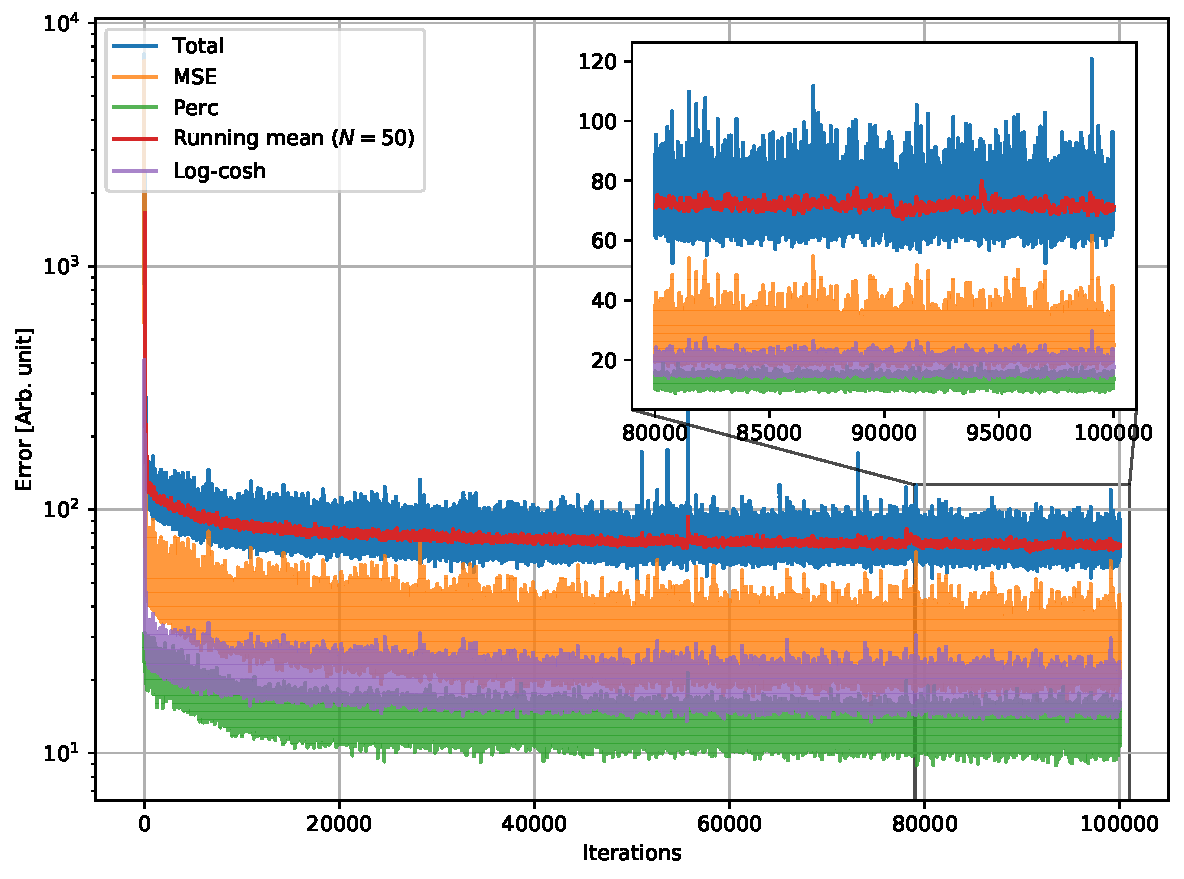
\includegraphics[width=.85\textwidth]{figures/losstomo00058ns32itd4mse035logcosh3depth1.pdf}
  \caption[Loss function evolution]{Loss function evolution. } 
  \label{fig:losstomo00058noadv}
\end{figure}


\section{TomoGAN Compared to PICCS}
\todo[]{Change section name?}
\todo[inline]{Axial, sagittal, coronal plots for different depth parameters. }
\todo[inline]{Maybe make 3D model plot of this dataset. }
\todo[inline]{Line plot comparing GT, FDK?, PICCS, denoised. }
\todo[inline]{Histogram. Looks like peaks roughly align, sharper peaks. Looks like it is performing segmentation? Note: ordinate (y-axis) cropped to 20k. }

\cref{fig:kimrobertcomparison,fig:sideplothq,fig:sideplotfdk,fig:sideplotpiccs,fig:sideplotdepth1,fig:sideplotdepth3,fig:sideplotdepth5,fig:sideplotdepth7,fig:kimrobertline,fig:kimroberthist}. 

\begin{figure}
    \begin{subfigure}[t]{.45\textwidth}
      \centering
      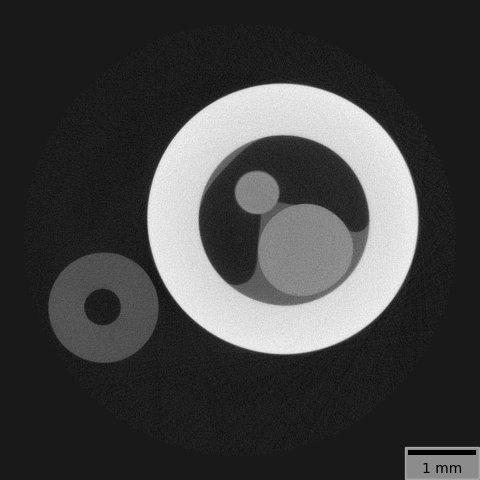
\includegraphics[width=\linewidth]{figures/kimrobertgt.png}
      \caption{High-quality FDK. }
    \end{subfigure}
    \hfill
    \begin{subfigure}[t]{.45\textwidth}
      \centering
      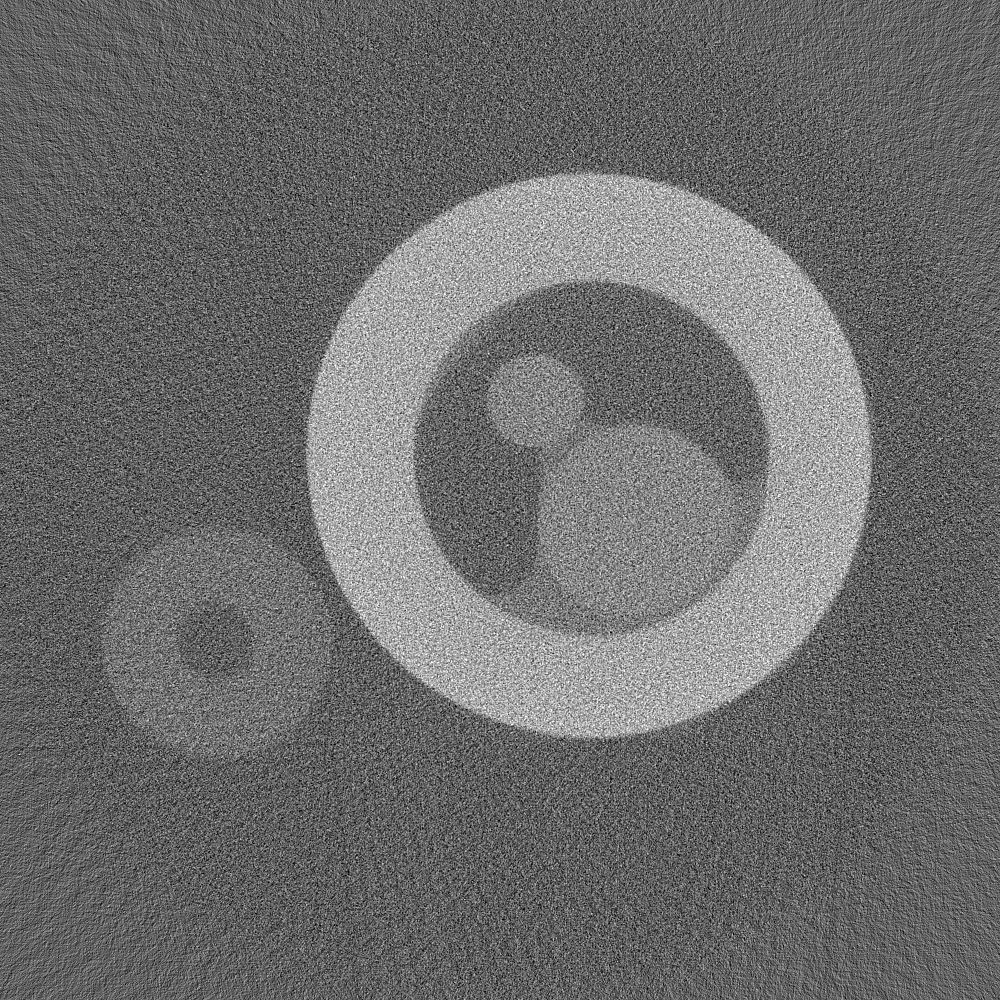
\includegraphics[width=\linewidth]{figures/kimrobertFDK.png}
      \caption{Low-quality FDK.}
    \end{subfigure}
  
    \medskip
  
    \begin{subfigure}[t]{.45\textwidth}
      \centering
      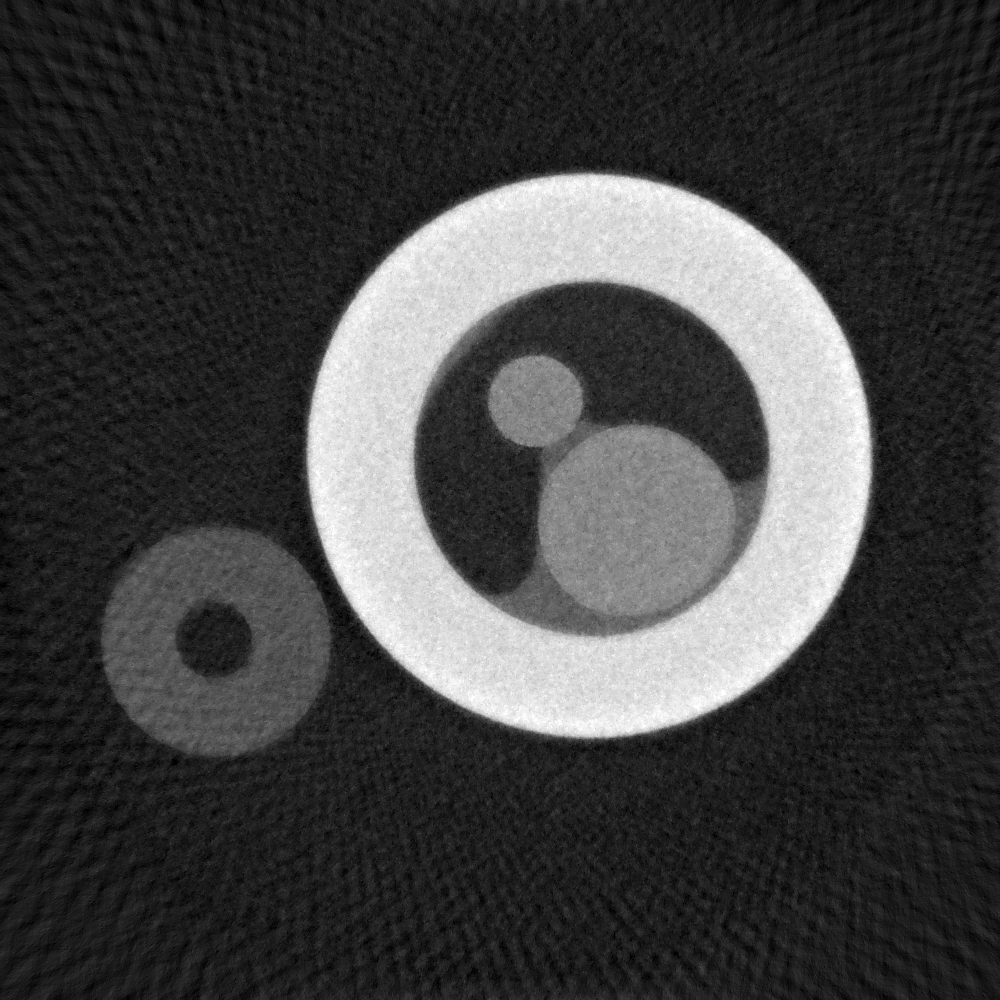
\includegraphics[width=\linewidth]{figures/kimrobertPICCS.png}
      \caption{\acrshort{piccs}. }
    \end{subfigure}
    \hfill
    \begin{subfigure}[t]{.45\textwidth}
      \centering
      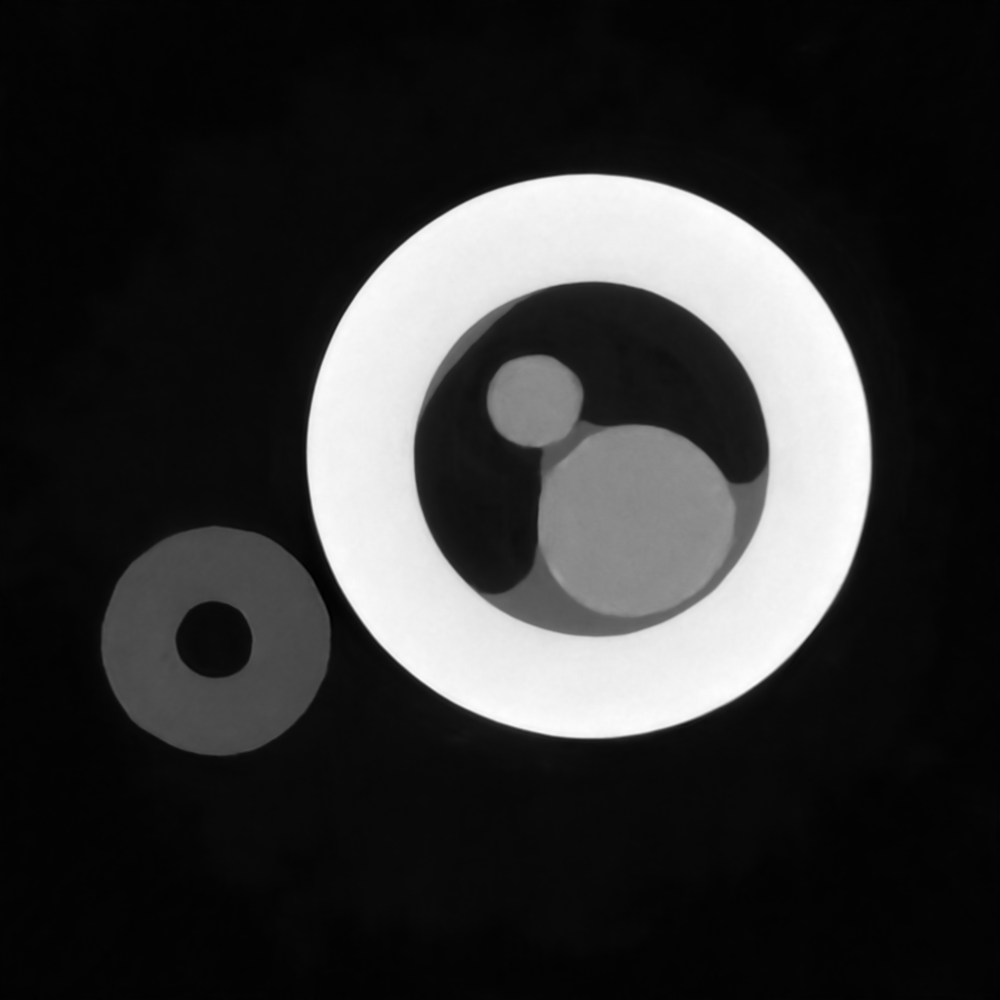
\includegraphics[width=\linewidth]{figures/kimrobertdepth1dn.png}
      \caption{FDK denoised. }
    \end{subfigure}
    \caption[Comparison of different reconstructions]{Comparison of different reconstructions. }
    \label{fig:kimrobertcomparison}
\end{figure}
\todo[]{Remove \cref{fig:kimrobertcomparison}? May not be needed, as this is basically showed in other figures. }

\begin{figure}[htbp]
  \centering
  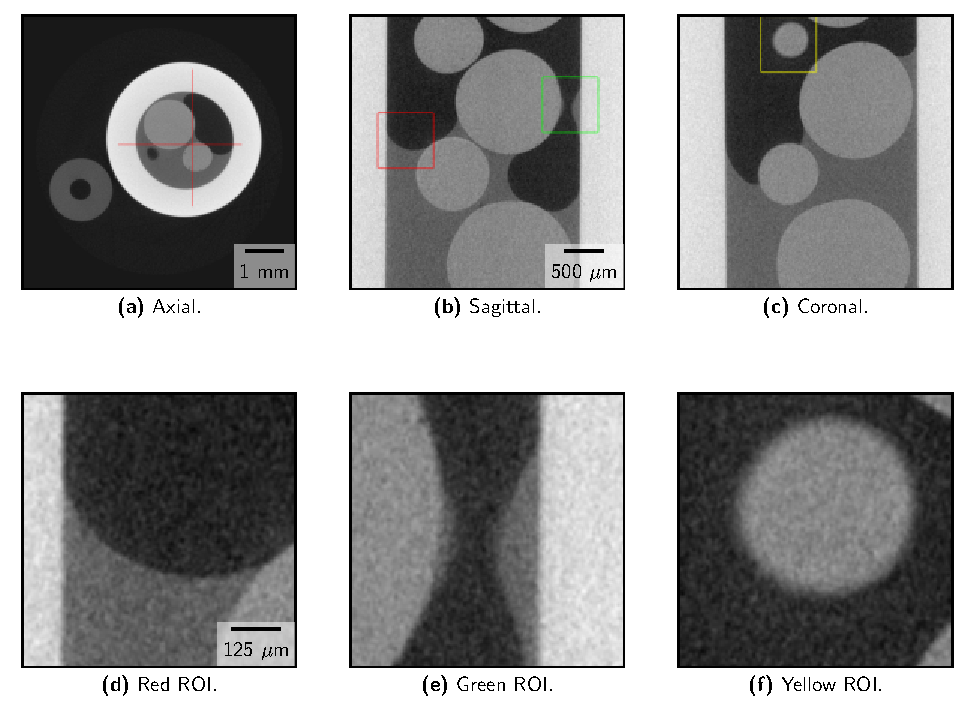
\includegraphics[width=.9\textwidth]{figures/kimroberthq-x475y620s250.pdf}
  \caption[High-quality]{View of the high-quality FDK reconstruction. The red horizontal line in \textbf{(a)} corresponds to the sagittal view in \textbf{(b)}, and the red vertical line corresponds to the coronal view in \textbf{(c)}. Three \acrshort{roi}s have been marked in \textbf{(b)} and \textbf{(c)}, and can be seen in \textbf{(d)}-\textbf{(f)}. }
  \label{fig:sideplothq}
\end{figure}

\begin{figure}[htbp]
  \centering
  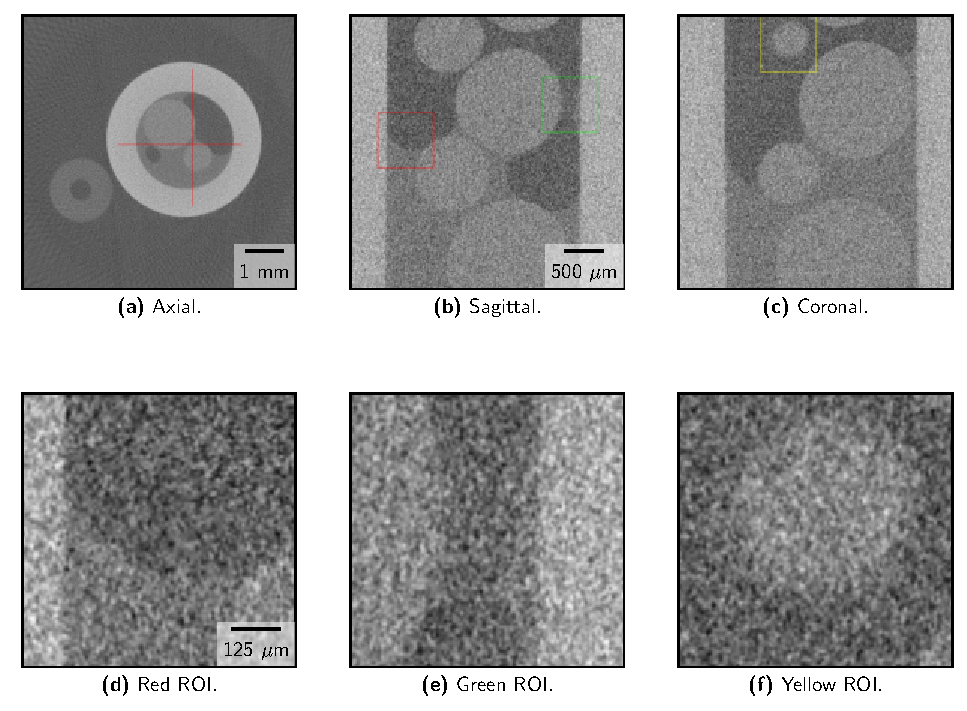
\includegraphics[width=.9\textwidth]{figures/kimrobertfdk-x475y620s250.pdf}
  \caption[FDK]{View of the low-quality FDK reconstruction. Figure elements are as in \cref{fig:sideplothq}.} 
  \label{fig:sideplotfdk}
\end{figure}

\begin{figure}[htbp]
  \centering
  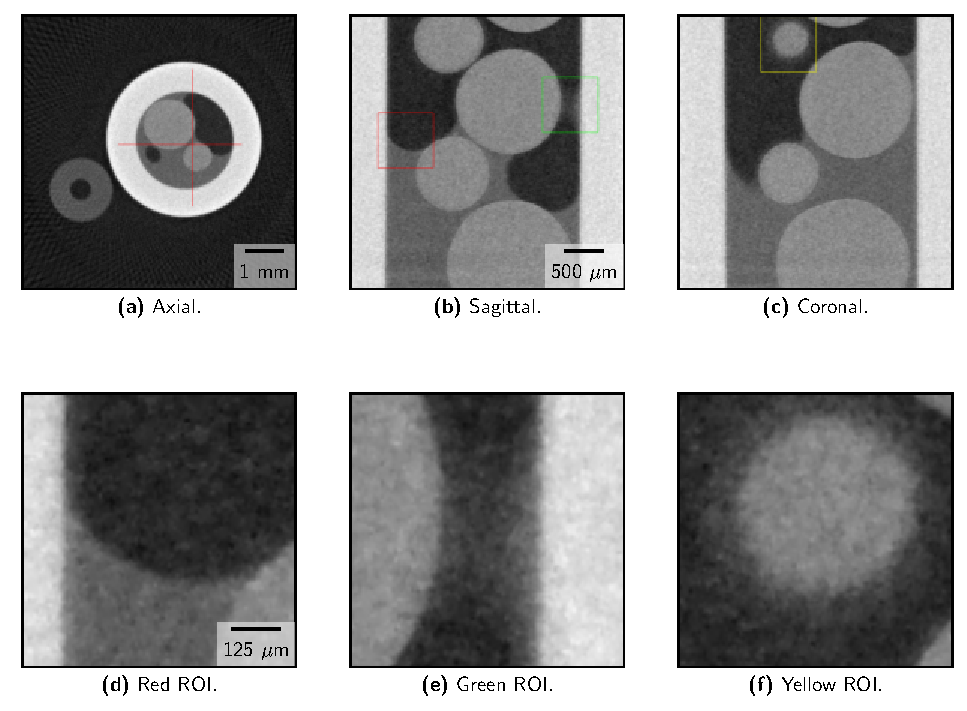
\includegraphics[width=.9\textwidth]{figures/kimrobertpiccs-x475y620s250.pdf}
  \caption[PICCS]{View of the \acrshort{piccs} reconstruction. Figure elements are as in \cref{fig:sideplothq}. }
  \label{fig:sideplotpiccs}
\end{figure}

\begin{figure}[htbp]
  \centering
  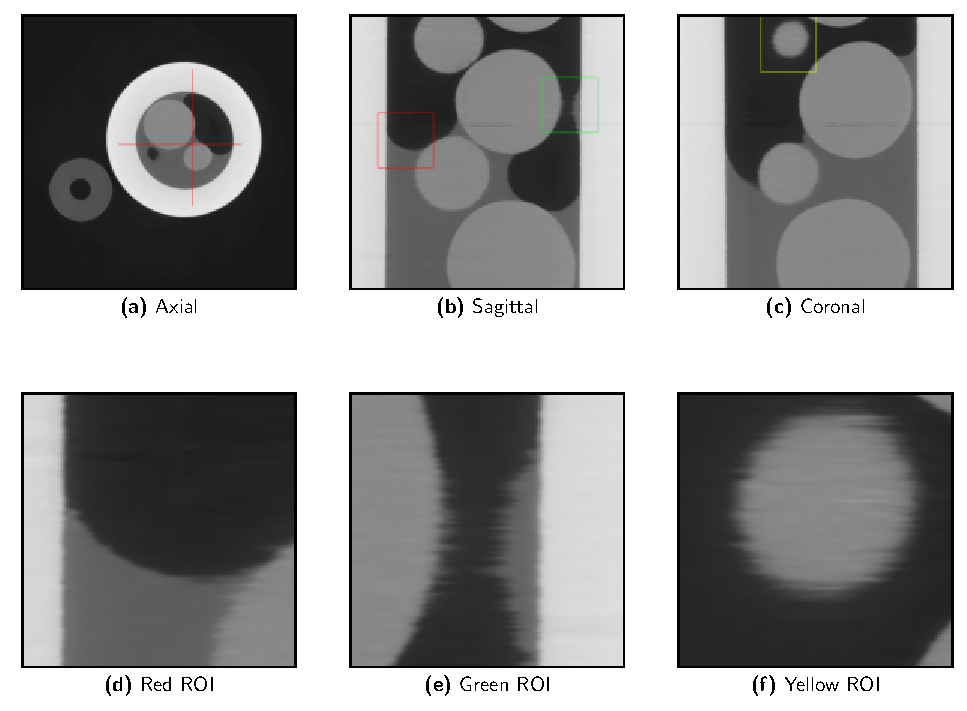
\includegraphics[width=.9\textwidth]{figures/kimrobertdepth1-x475y620s250.pdf}
  \caption[Depth=1]{View of the denoised FDK reconstruction with a depth of 1. Figure elements are as in \cref{fig:sideplothq}. }
  \label{fig:sideplotdepth1}
\end{figure}

\begin{figure}[htbp]
  \centering
  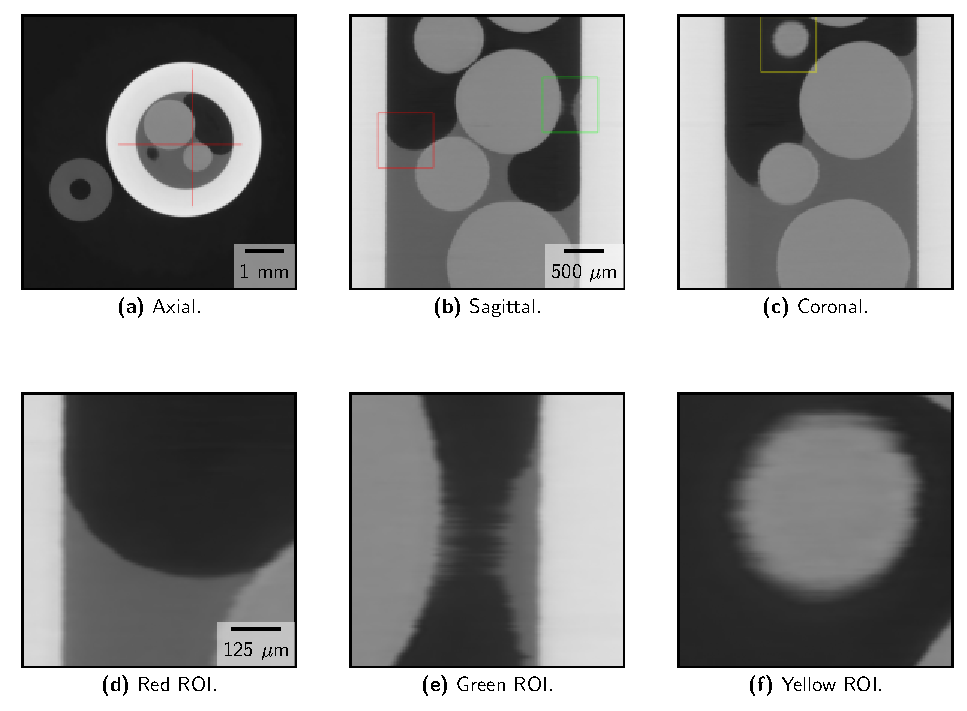
\includegraphics[width=.9\textwidth]{figures/kimrobertdepth3-x475y620s250.pdf}
  \caption[Depth=3]{View of the denoised FDK reconstruction with a depth of 3. Figure elements are as in \cref{fig:sideplothq}. }
  \label{fig:sideplotdepth3}
\end{figure}

\begin{figure}[htbp]
  \centering
  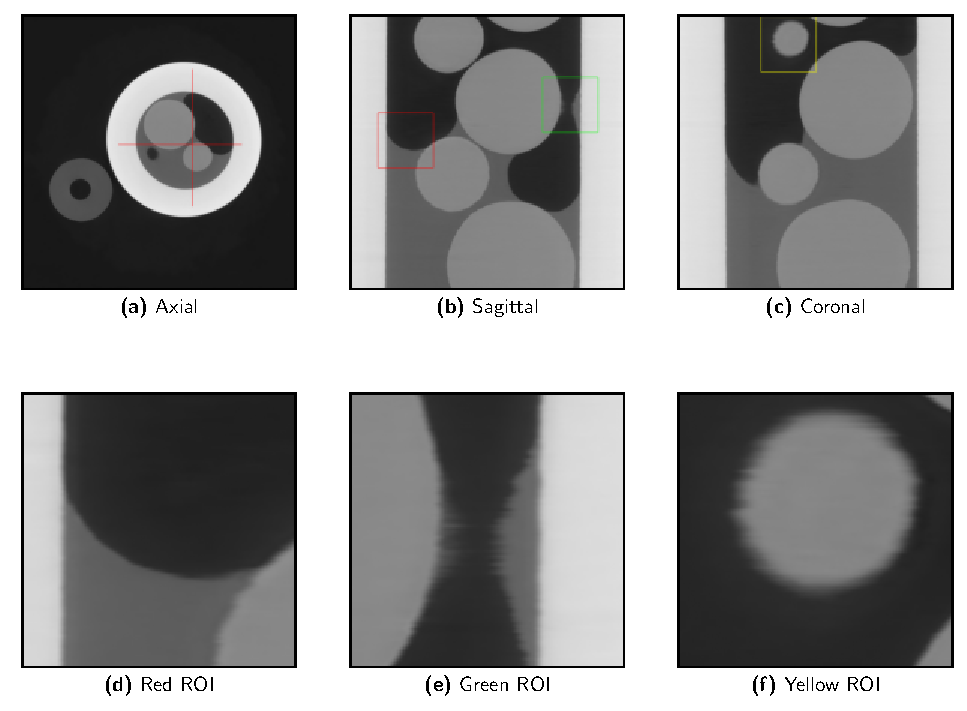
\includegraphics[width=.9\textwidth]{figures/kimrobertdepth5-x475y620s250.pdf}
  \caption[Depth=5]{View of the denoised FDK reconstruction with a depth of 5. Figure elements are as in \cref{fig:sideplothq}. }
  \label{fig:sideplotdepth5}
\end{figure}

\begin{figure}[htbp]
  \centering
  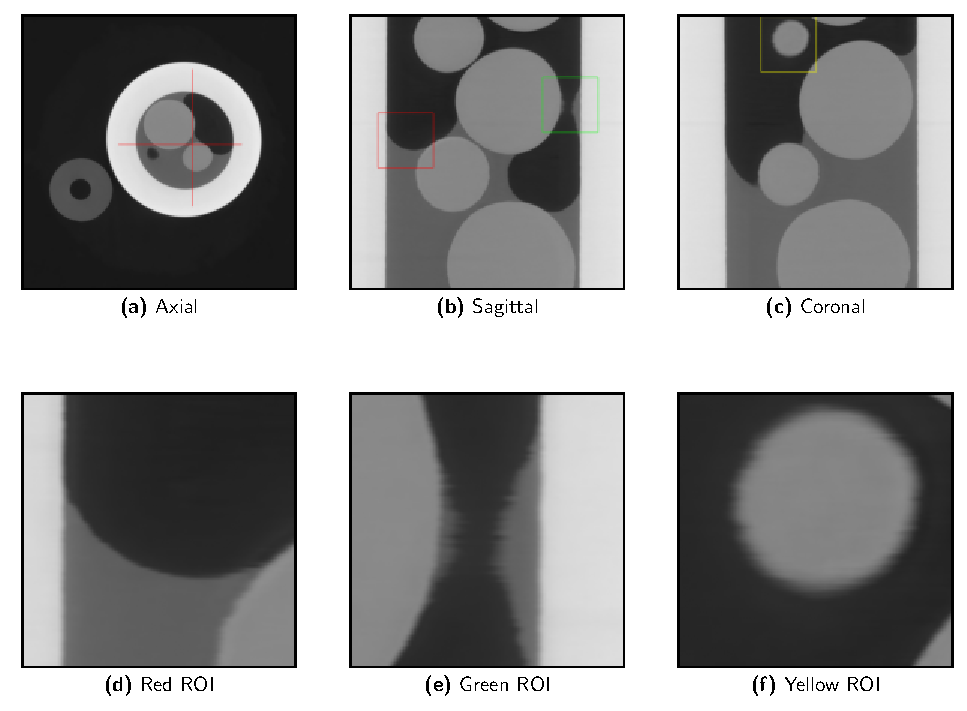
\includegraphics[width=.85\textwidth]{figures/kimrobertdepth7-x475y620s250.pdf}
  \caption[Depth=7]{View of the denoised FDK reconstruction with a depth of 7. Figure elements are as in \cref{fig:sideplothq}. }
  \label{fig:sideplotdepth7}
\end{figure}

\begin{figure}[htbp]
  \centering
  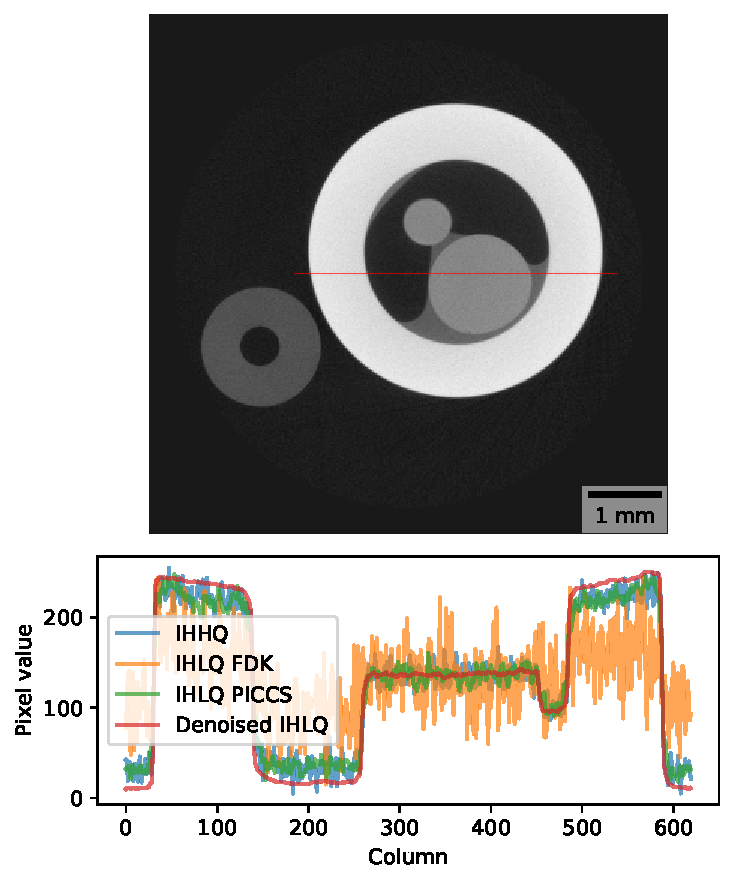
\includegraphics[width=.85\textwidth]{figures/kimrobertline.pdf}
  \caption[Line plot]{The plot shows pixel values for 620 pixels on a horizontal line, as shown by the red line on the high-quality image above. The denoised values are from denoising the FDK reconstruction with TomoGAN using a loss function containing \acrshort{mse}, log-cosh, VGG, and adversarial loss components, a depth of 1, and the network was trained for $100 000$ iterations. }
  \label{fig:kimrobertline}
\end{figure}

\begin{figure}[htbp]
  \centering
  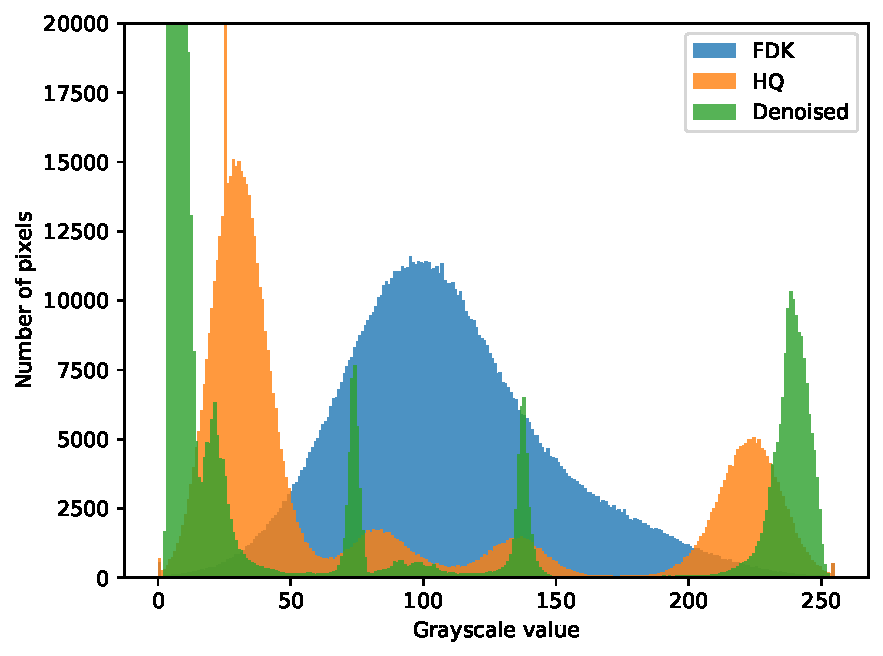
\includegraphics[width=.85\textwidth]{figures/kimroberthist.pdf}
  \caption[Histogram]{Histograms of different reconstructions, including a denoising of the FDK reconstruction. The denoising was done with TomoGAN using a loss function containing \acrshort{mse}, log-cosh, VGG, and adversarial loss components, a depth of 1, and the network was trained for $100 000$ iterations. Note that the ordinate has been cropped to a max value of $20000$. }
  \label{fig:kimroberthist}
\end{figure}

\section{Attempted Shale Denoising}
\todo[inline]{Shows limitations of method: requires a high-quality similar dataset (i.e. some ground truth) to work properly. Any given trained network doesn't work for all other dataset. }
\cref{fig:shale}

\begin{figure}
  \begin{subfigure}[t]{\textwidth}
    \centering
    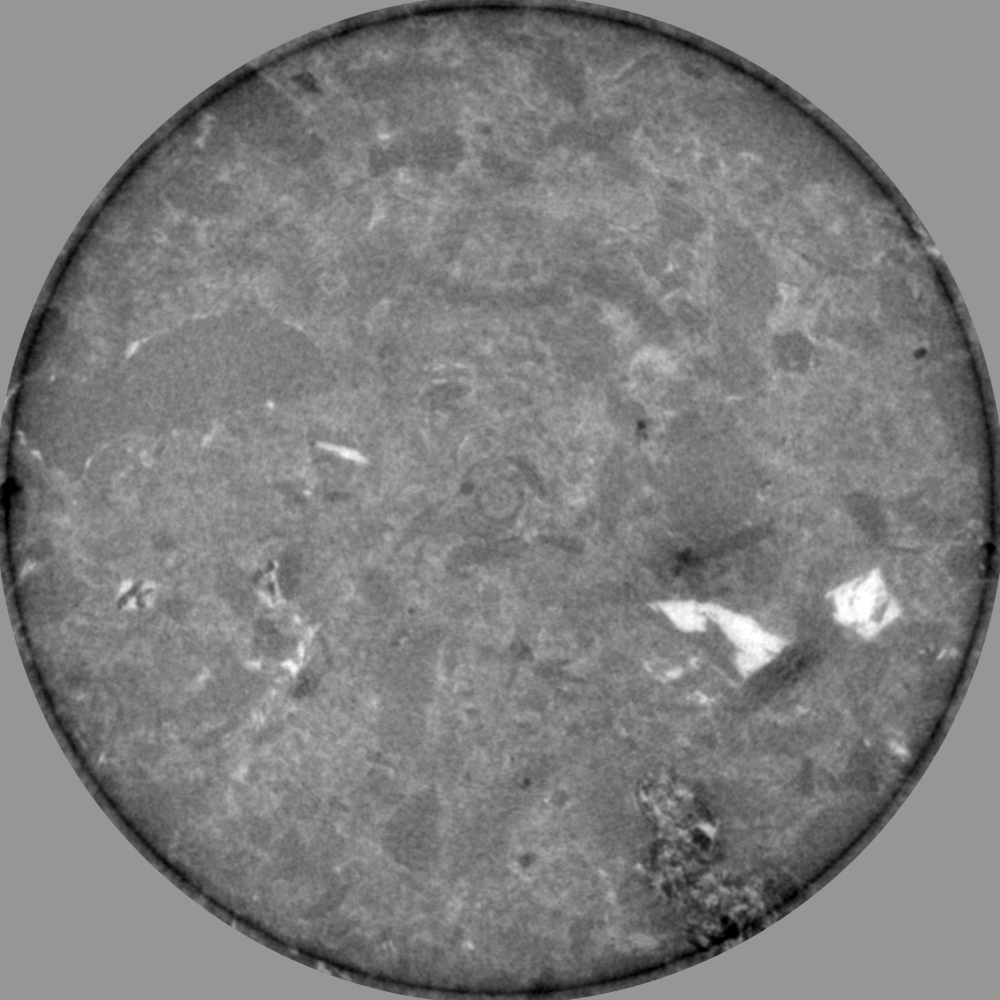
\includegraphics[width=.45\textwidth]{figures/shale/shale_ns/0.png}
    \caption{Original image. }
  \end{subfigure}

  \medskip

  \begin{subfigure}[t]{.45\textwidth}
    \centering
    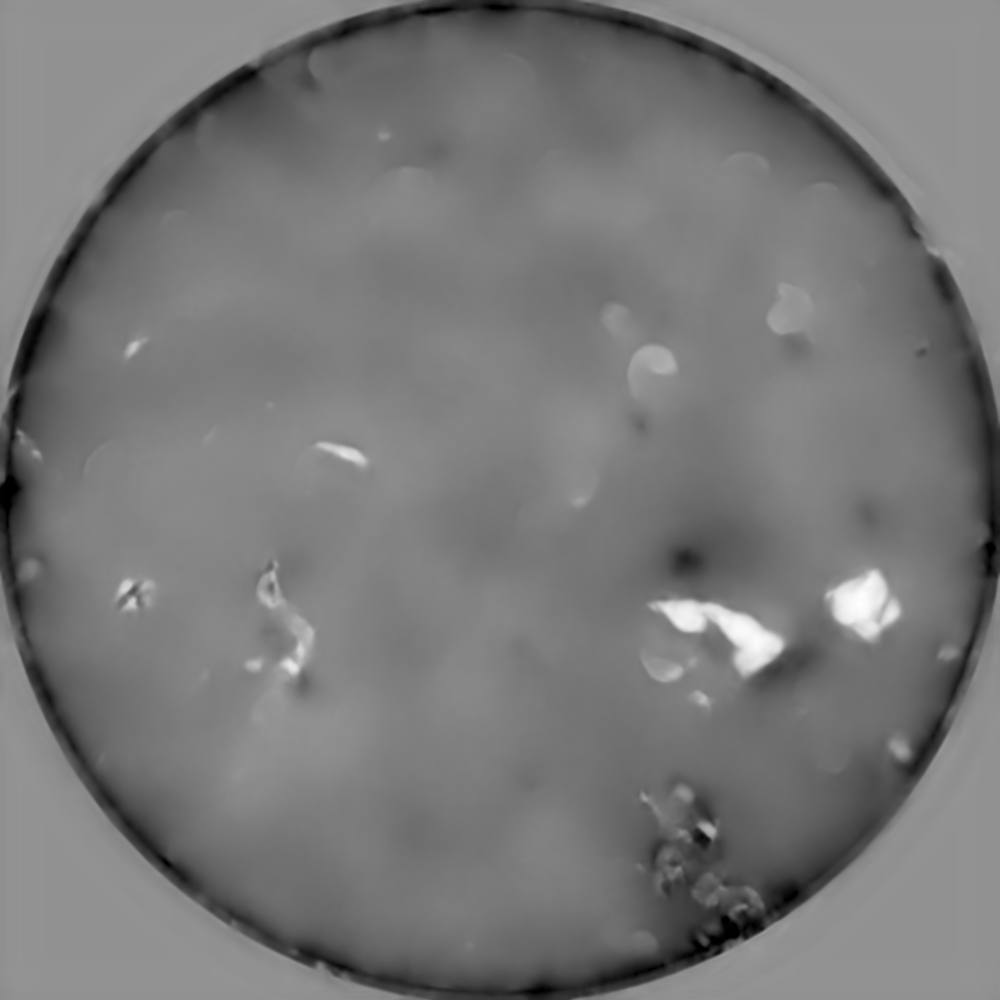
\includegraphics[width=\linewidth]{figures/shale/shale_dn_tomo00058/0.png}
    \caption{tomo\_00058. }
  \end{subfigure}
  \hfill
  \begin{subfigure}[t]{.45\textwidth}
    \centering
    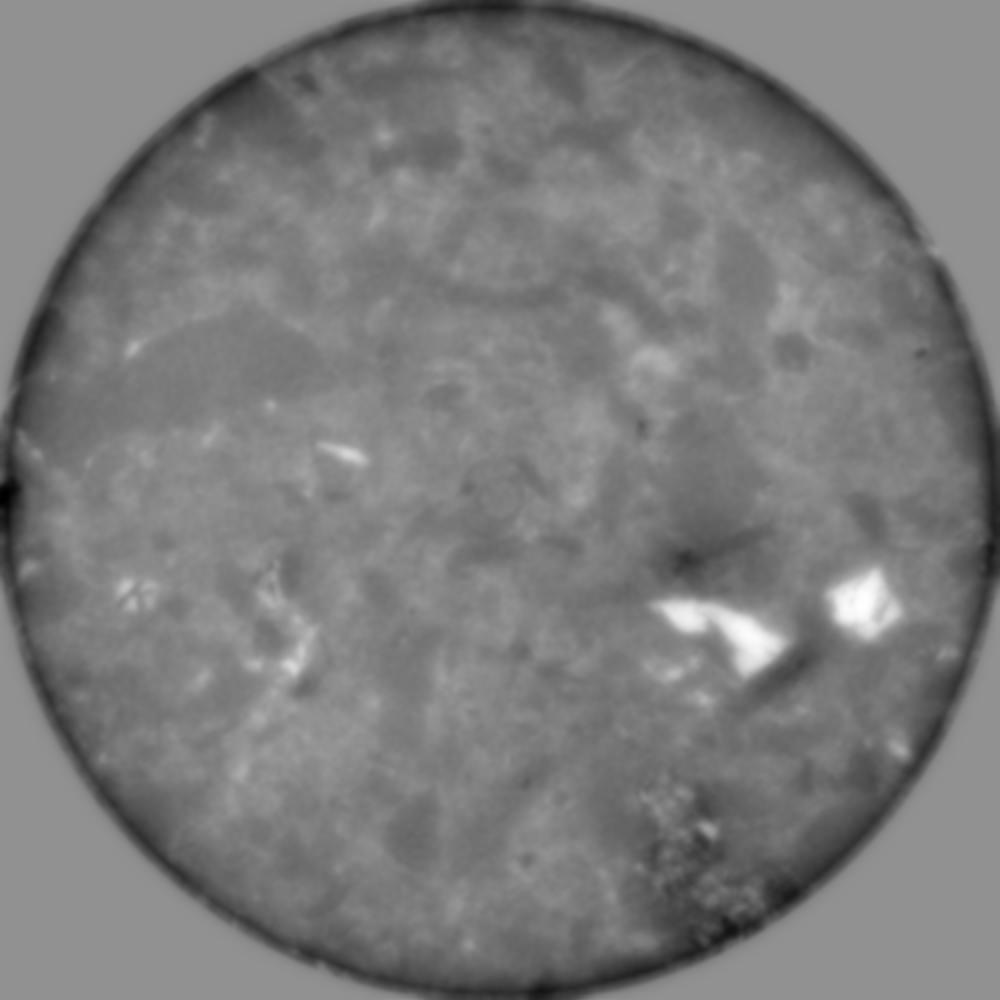
\includegraphics[width=\linewidth]{figures/shale/shale_dn_tomo00001/0.png}
    \caption{tomo\_00001. }
  \end{subfigure}

  \medskip

  \begin{subfigure}[t]{.45\textwidth}
    \centering
    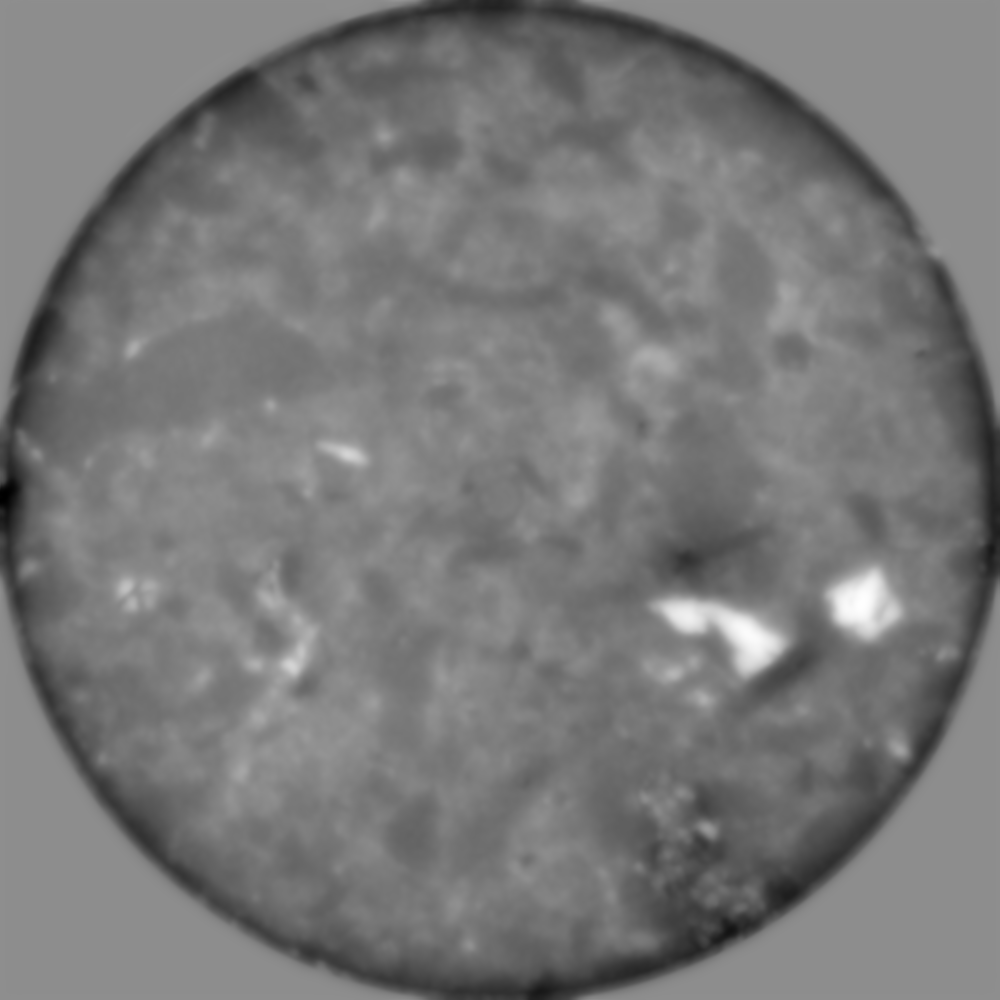
\includegraphics[width=\linewidth]{figures/shale/shale_dn_tomo00002/0.png}
    \caption{tomo\_00002. }
  \end{subfigure}
  \hfill
  \begin{subfigure}[t]{.45\textwidth}
    \centering
    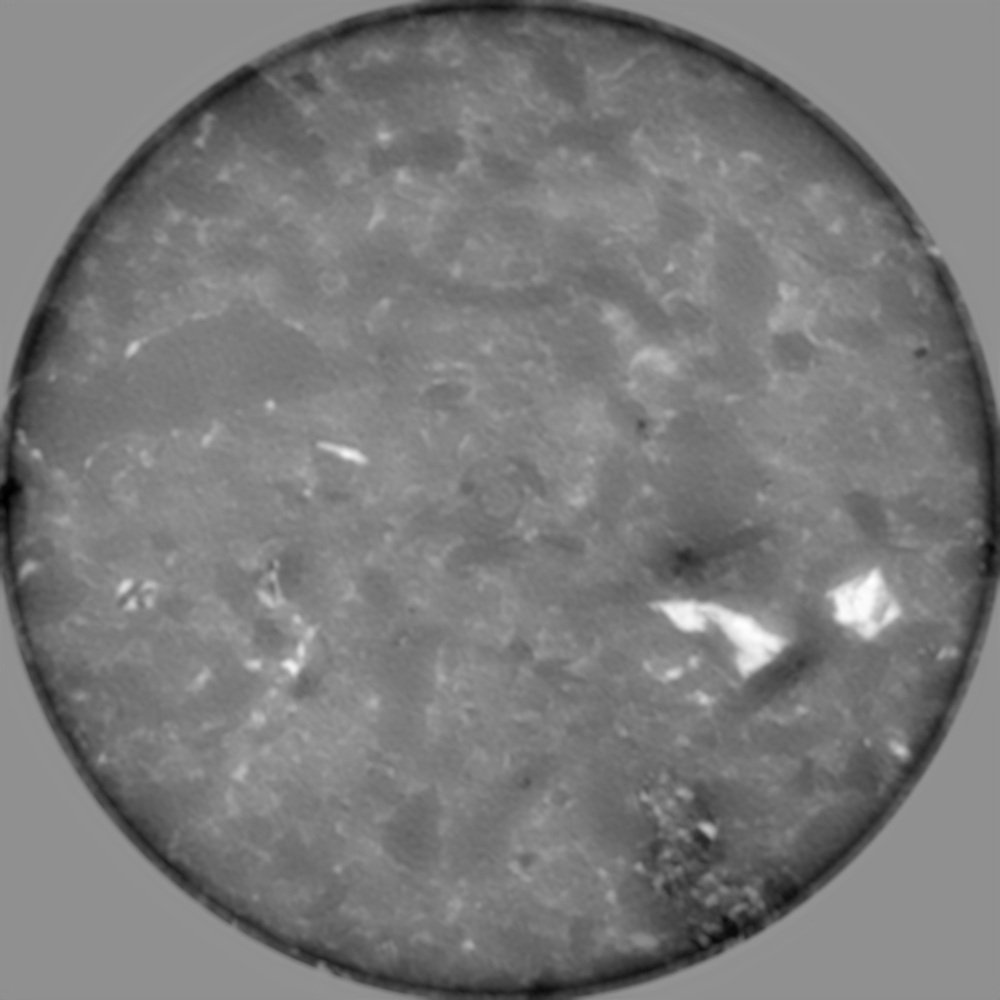
\includegraphics[width=\linewidth]{figures/shale/shale_dn_tomo00002min7/0.png}
    \caption{tomo\_00002min7. }
  \end{subfigure}
  \caption[Attempted shale denoising]{Attempted shale denoising. }
  \label{fig:shale}
\end{figure}




%Plot types: 
%\begin{itemize}
%    \item \acrshort{ssim} and \acrshort{mse} changes during training.
%    \item Loss function evolution.
%    \item Line plot of gt, ns, and different loss functions?
%    \item Histograms of gt, ns, denoised
%    \item Zoomed in region of interest.
%    \item Axial, sagittal, and coronal plots of (at least Kim Robert's dataset) different depth parameters.
%    \item Compare denoising of different subsamplings (8, 16, 32, 48)
%    \item Activation plot of network layers.
%\end{itemize}